\capitulo{5}{Aspectos relevantes del desarrollo del proyecto}

En este apartado se va a comentar el desarrollo que ha tenido el proyecto. Se expondrán todas las líneas de investigación seguidas, cuál ha sido el problema de cada una y las posibles soluciones.

\section{Inicio del proyecto}

Este proyecto comenzó como un proyecto de investigación sobre la extracción de secuencias mediante el algoritmo \textbf{Dynamic Time Warping}. Las secuencias a investigar debían de ser obtenidas mediante un proyecto fin de máster creado por los alumnos José Luís Garrido Labrador y José Miguel Ramírez Sanz. 

Por esta razón inicialmente el proyecto no tenía un objetivo concreto más allá de la extracción de las posiciones a partir del proyecto anteriormente mencionado y el análisis de dichas secuencias. 

Tras realizar numerosos vídeos y obtener secuencias a partir de distintos puntos del esqueleto humano, se planteó como objetivo principal la localización de ejercicios concretos dentro de secuencias de mayor tamaño y su posterior clasificación según las extremidades del cuerpo que el paciente ejercitase.  

\section{Investigación del proceso a seguir}

Una vez establecido el objetivo del proyecto, el proceso a seguir fue el que se puede observar en la figura \ref{fig:diagramP}: procesar cada uno de los vídeos almacenados, de cada vídeo obtener una descomposición de todos y cada uno de los \textit{frames} que lo componen, de cada \textit{frame} obtener el esqueleto del paciente o terapeuta, almacenar las posiciones del esqueleto, y finalmente analizar y clasificar dichas posiciones. Una vez conocido el proceso a seguir, surgen numerosas cuestiones acerca del mismo: ¿De dónde se van a obtener los vídeos? ¿Qué cantidad de posiciones se precisa almacenar? ¿Qué medios se van a usar para clasificar las secuencias? ¿Qué se considerará un buena clasificación?

\begin{figure}[H]
    \centering
    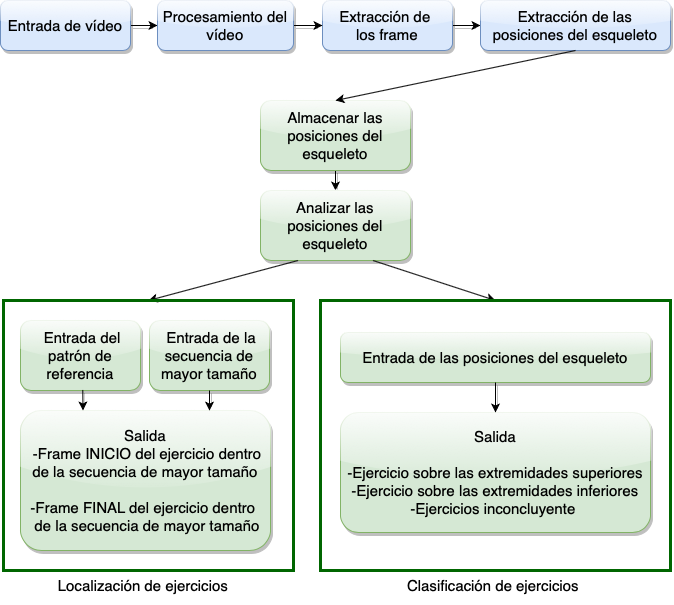
\includegraphics[width=\textwidth]{plantillaLatex-master/img/DiagramProyect.png}
    \caption{Diagrama del flujo del proyecto.}
    \label{fig:diagramP}
\end{figure}

Cabe destacar que como se trata de un proyecto de investigación sobre como sacar información de diferentes vídeos, los resultados obtenidos están influenciados por el tipo de vídeos que se han aportado. 

A la hora de responder a las anteriores cuestiones propuestas, se ha hecho una minuciosa investigación sobre múltiples artículos publicados que emplean técnicas similares para el fin planteado. En concreto en el apartado \textit{trabajos relacionados} \ref{cap:TrabRelTaiChi}, un grupo de investigadores del \textit{Instituto Avanzado de Ciencias de Corea y Technology (KAIST)} realizan un estudio sobre como detectar movimientos de \textit{Tai Chi} utilizando como medida de reconocimiento la distancia \textbf{DTW}. Este estudio, que ha sido realizado sobre 21 sujetos, cuenta con las siguientes características: 
\begin{enumerate}
    \item Realiza comparaciones sobre poses en 3D, para ello obtiene las coordenadas $X, Y, Z$ de las diferentes articulaciones y posiciones de los huesos. Para este proyecto, inicialmente se propuso hacerlo con dichas dimensiones pero se descartó rápidamente por la elevada cantidad de tiempo que requerían las ejecuciones.
    \item Compara los movimientos redimensionando las series temporales en series unidimensionales, esta característica si que ha sido implantada en este proyecto por los buenos resultados que arroja.
    \item Calcula el desplazamiento entre movimientos, es decir, calcula la diferencia que ejerce una extremidad entre el \textit{frame} actual y el \textit{frame} inmediatamente anterior. En este proyecto no se ha calculado la diferencia entre posiciones, pero queda propuesto como líneas futuras realizar un cálculo sobre la diferencia de posiciones y en cuestión del valor obtenido poder encontrar la secuencia de referencia. 
\end{enumerate}

Por ello se llegó a la siguiente conclusión, como primera partida sobre la búsqueda de secuencias mediante \emph{DTW} no es necesario disponer de una amplia cantidad de vídeos, si no, en su defecto, realizar vídeos con una amplia similitud entre los ejercicios que los componen y ver como responde el algoritmo. 

Una vez realizados los vídeos con distintos ejercicios en ellos había numerosos factores a tener en cuenta, como: comprobar las características de las posiciones de cada esqueleto, como varían las posiciones entre los diferentes ejercicios, comprobar las diferencias entre las articulaciones que están en movimiento y las que supuestamente deberían de permanecer inmóviles. Este último factor es decisivo en la correcta localización de la secuencia. Por ejemplo, en un movimiento sobre las extremidades superiores está claro que las posiciones relativas a éstas van a tener una \texttt{desviación típica}\footnote{Mide la dispersión entre un conjunto de datos numéricos} mucho mayor que las relativas a las extremidades inferiores, pero la cuestión es ¿cómo de diferentes serán esos datos?. Puede que si un paciente realiza ejercicios sobre las extremidades superiores y acaba moviendo las extremidades inferiores, por ejemplo, porque está de pie y se cansa o le cuesta mantener el equilibrio, esta diferencia de posiciones afectará directamente a la localización de la secuencia.

Finalmente, también se realizaron numerosas pruebas sobre que tipo de datos utilizar. Se empezó utilizando un conjunto de datos de tres dimensiones, más adelante se cambió por conjuntos de datos unidimensionales que contenían las posiciones relativas a los ángulos del esqueleto y seguidamente se probó con datos bidimensionales que contenían todas las posiciones extraídas del esqueleto y los ángulos anteriormente comentados. Como se ha especificado, los ángulos son valores unidimensionales por lo que para la correcta comparación de secuencias al ser añadidos a las posiciones bidimensionales del esqueleto, se les tuvo que añadir una segunda dimensión. Esta segunda dimensión fue creada añadiendo un valor de cero en la posición relativa al eje $Y$. Para la búsqueda de secuencias no es ningún impedimento porque todas las secuencias, tanto las de referencia como la secuencia de mayor tamaño en la que se busca el patrón, tendrían un cero extra en las posiciones $Y$ de los ángulos, por lo que para encontrar similitudes no causaría estragos. Por otra parte si los causaría si lo que se pretende es representar el esqueleto, ya que en este caso localizaría cada uno de los ángulos en una posición del eje $X$ pero siempre en la misma del eje $Y$, la posición cero.


\section{Conjunto de Vídeos} \label{cap:Cvideos}

Inicialmente el conjunto de vídeos iba a ser aportado por pacientes y terapeutas pero como éstos se demoraban se optó por realizar los vídeos personalmente. Los vídeos con los que se han realizado todas las pruebas son vídeos realizados por tres individuos, uno de ellos la autora del proyecto con sexo femenino y 24 años de edad y los restantes, con un total de dos compañeros, con sexo masculino y 23 años de edad. 

Como el objetivo principal de este proyecto es localizar secuencias de movimientos y no evaluarlas, el quien realice los vídeos no es un gran impedimento para lograr el objetivo, lo que si que puede suponer es una falsa esperanza de poder aplicar las técnicas descubiertas a pacientes reales. Todos los individuos con los que se han realizado las pruebas son individuos sanos y jóvenes por lo que los movimientos tienden a ser precisos. Es por esta razón que al no haberse probado con vídeos de pacientes reales no se puede garantizar su funcionamiento en personas con trastornos neurológicos. 

Otro aspecto a tener en cuenta es el tipo de movimientos realizados. En los vídeos se han realizado ejercicios cortos y asequibles a personas con la enfermedad de \textit{Parkinson}. Todos los ejercicios muestran movimientos en alguna de las extremidades del cuerpo y son ejercicios cortos para que se puedan realizar sin pausas una vez iniciado el movimiento. De todas formas estos ejercicios han sido propuestos por la autora del proyecto y no son ejercicios establecidos por un terapeuta. 

Finalmente comentar que todos los vídeos aportados se han realizado con consentimiento de los voluntarios y han accedido a que puedan ser utilizados para este proyecto. 


\section{Definición del problema} \label{cap:defProblem}

Este apartado consistirá en explicar a grandes rasgos en que ha consistido la búsqueda de secuencias. El primer aspecto a tener en cuenta es la longitud de las mismas. En la figura \ref{fig:skeletonFrame} se muestra un ejemplo del problema a plantear. Si tenemos una secuencia de ejercicios provenientes de un paciente, y otra misma secuencia de ejercicios pero en este caso realizados por un terapeuta, es demasiado improbable que ambas secuencias cuenten con la misma longitud. Es por esta razón que se ha elegido la búsqueda mediante \textbf{DTW}, que como se ha comentado en el apartado \ref{cap:DTW}, busca una alineación óptima entre secuencias de distinto tamaño. 


En la figura \ref{fig:skeletonFrame} se puede observar como ambas secuencias de esqueletos realizan el mismo movimiento. Según esa figura se puede observar como en la primera secuencia se obtiene un mayor número de esqueletos y por ende una secuencia de una longitud mayor. Esto puede ser provocado por la velocidad del movimiento, si los movimientos son más lentos, capturará un mayor número de \textit{frames} relativos a ese ejercicio. Este ejemplo es simplemente una idea visual para adentrarse en la raíz del problema que se va a plantear a continuación. 

\begin{figure}[H]
    \centering
    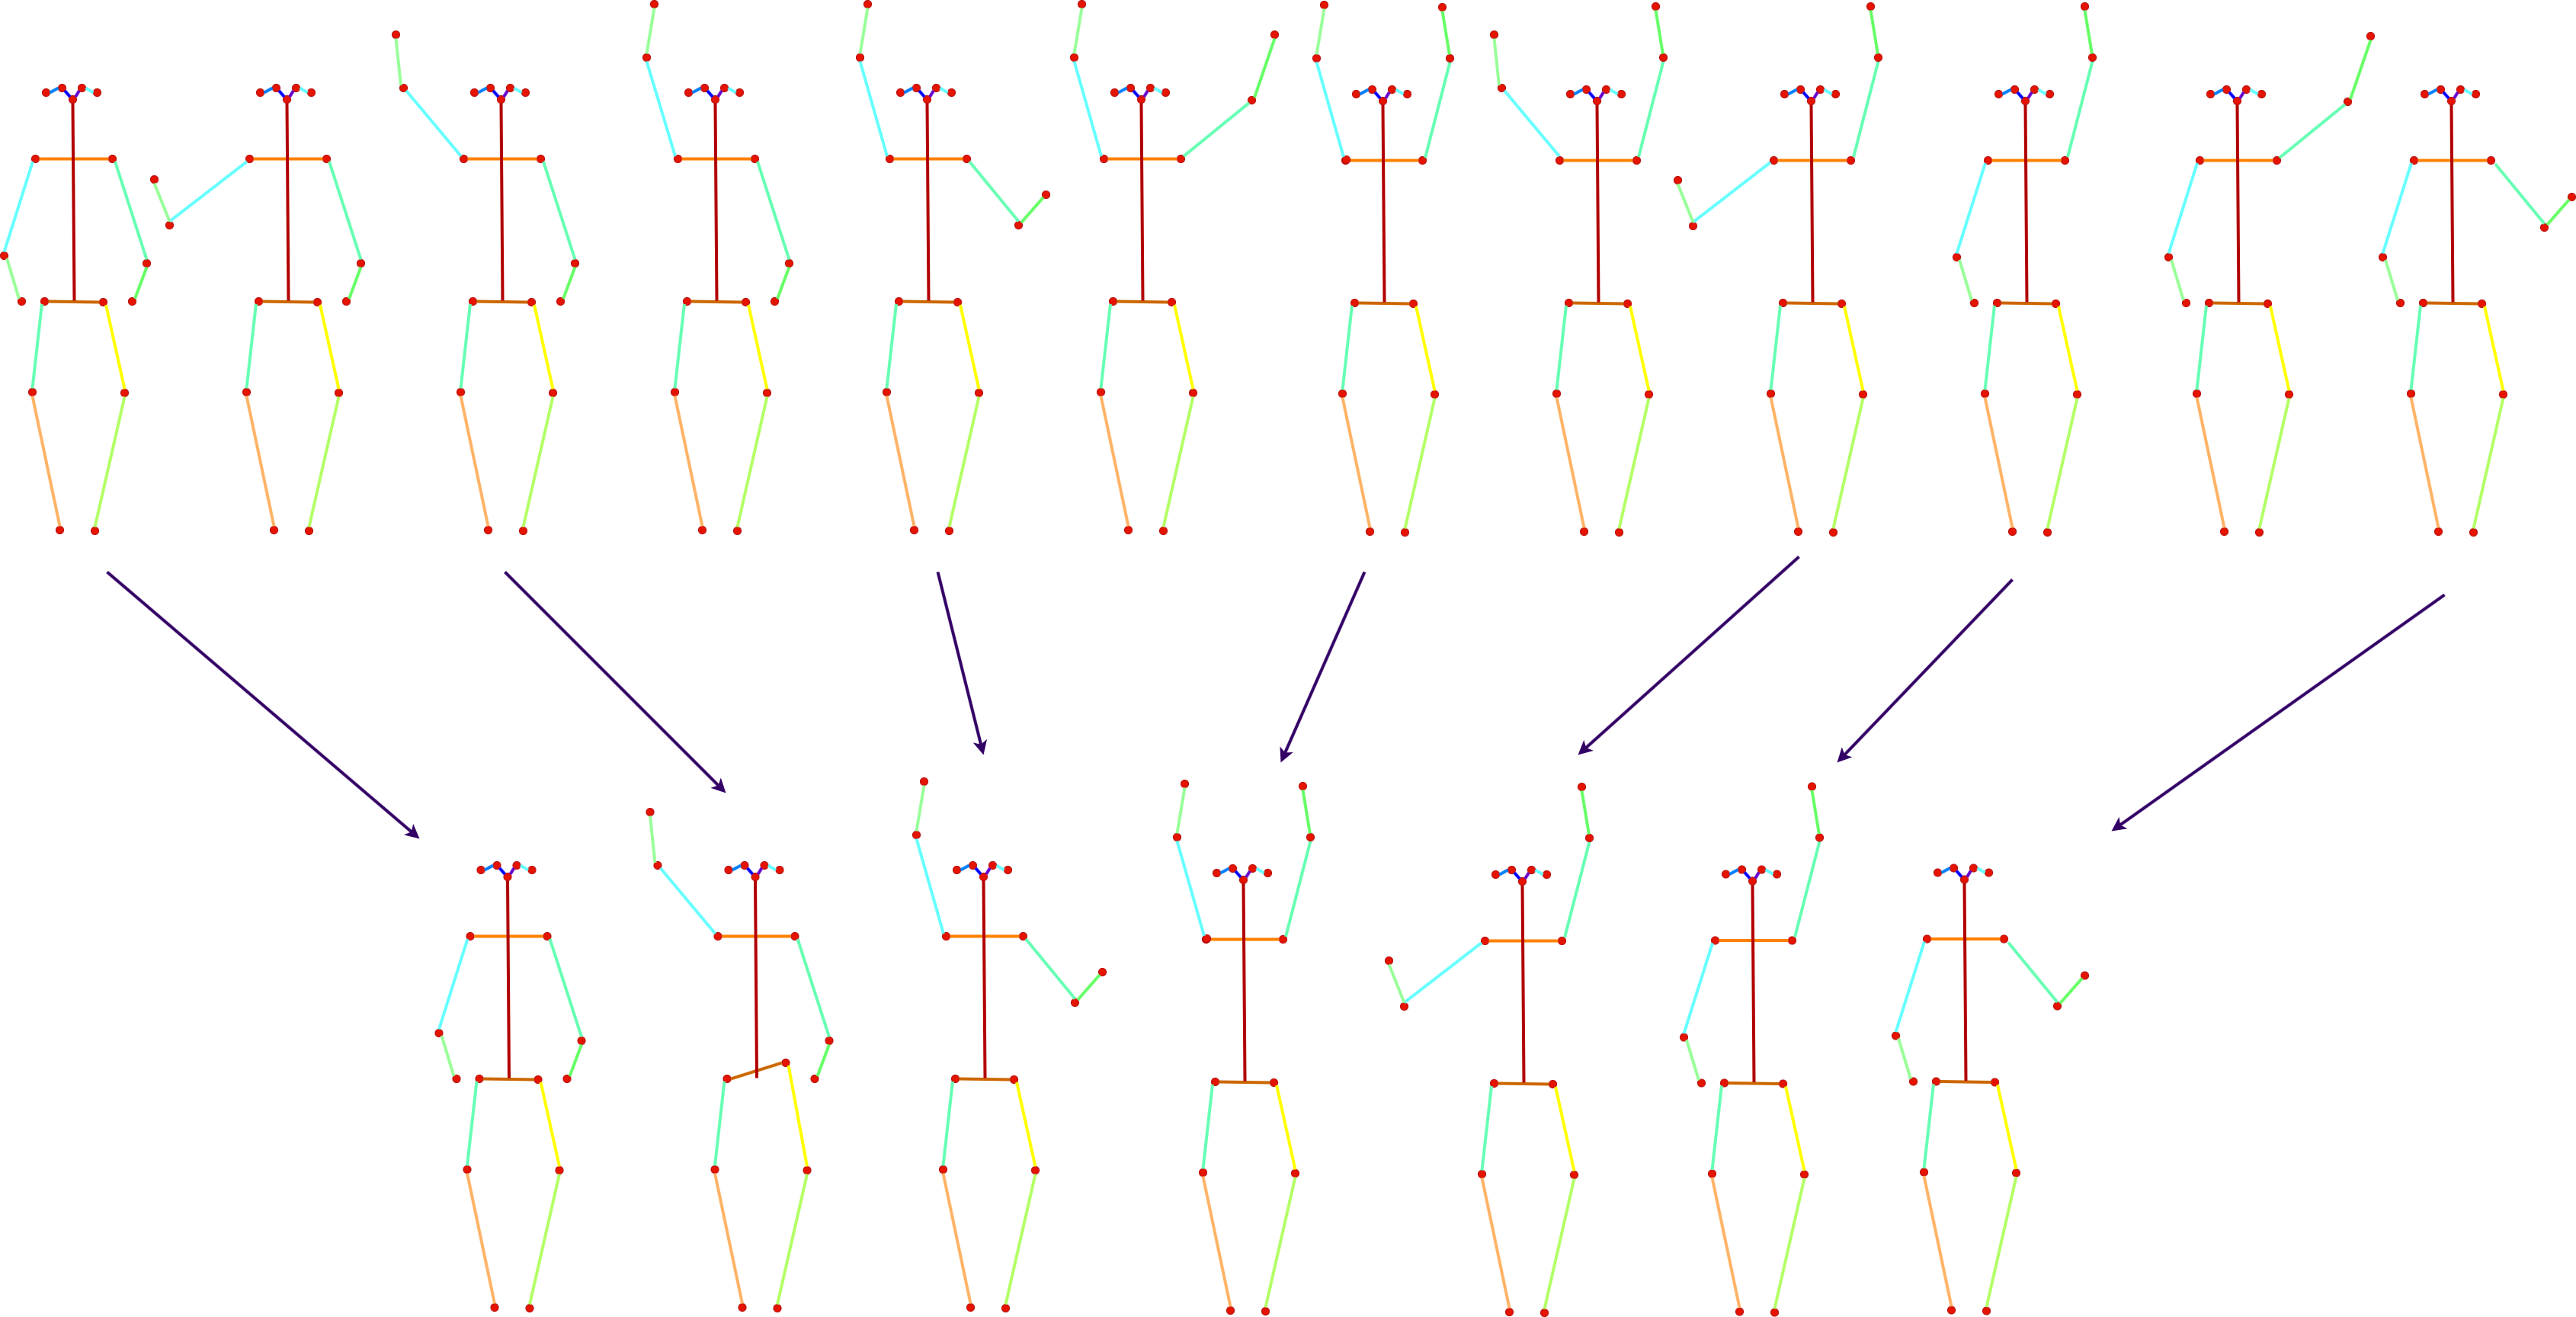
\includegraphics[width=\textwidth]{plantillaLatex-master/img/skeleton2.png}
    %Skeletons_frame.png}
    \caption{Alineación de esqueletos.}
    \label{fig:skeletonFrame}
\end{figure}

Por lo tanto, el problema principal será la búsqueda de la secuencia de ejercicios completa sin que la longitud de la secuencia sea un problema a la hora de realizar la búsqueda. Parece que con \emph{DTW} este problema está solucionado pero en el siguiente apartado se mostrarán algunos de los problemas obtenidos y sus posibles soluciones.

Otro problema a tener en cuenta son los movimientos involuntarios que puede realizar un paciente o individuo.Un ejercicio idóneo de movimientos sobre las extremidades superiores del cuerpo sería el que muestra la imagen \ref{f:f_esq_}. En esta imagen se puede observar como el paciente mueve únicamente los brazos dejando inmóviles el resto de partes de su cuerpo.

Lógicamente este es un ejemplo simulado que se ha creado para mostrar la dificultad de la búsqueda de secuencias. Por una parte, aunque el paciente se esté lo más concentrado posible en hacer correctamente su ejercicio, es imposible que realice el ejercicio exactamente igual al del terapeuta, pero sobretodo, es muy probable que mueva otras extremidades o partes del cuerpo involuntariamente, o como consecuencia de no mantener un correcto equilibrio. Tanto si se trata de un paciente con la enfermedad de \textit{Parkinson}, o de algún otro individuo, como pueden ser algunos de los lectores de este proyecto, si intentan realizar un ejercicio sobre las extremidades superiores del cuerpo, se acabarán dando cuenta de que en algún momento han movido un pie, la rodilla o han cambiado su posición, sobretodo si se trata de un ejercicio que se realiza de pie.
\begin{figure}[H]
    \centering
    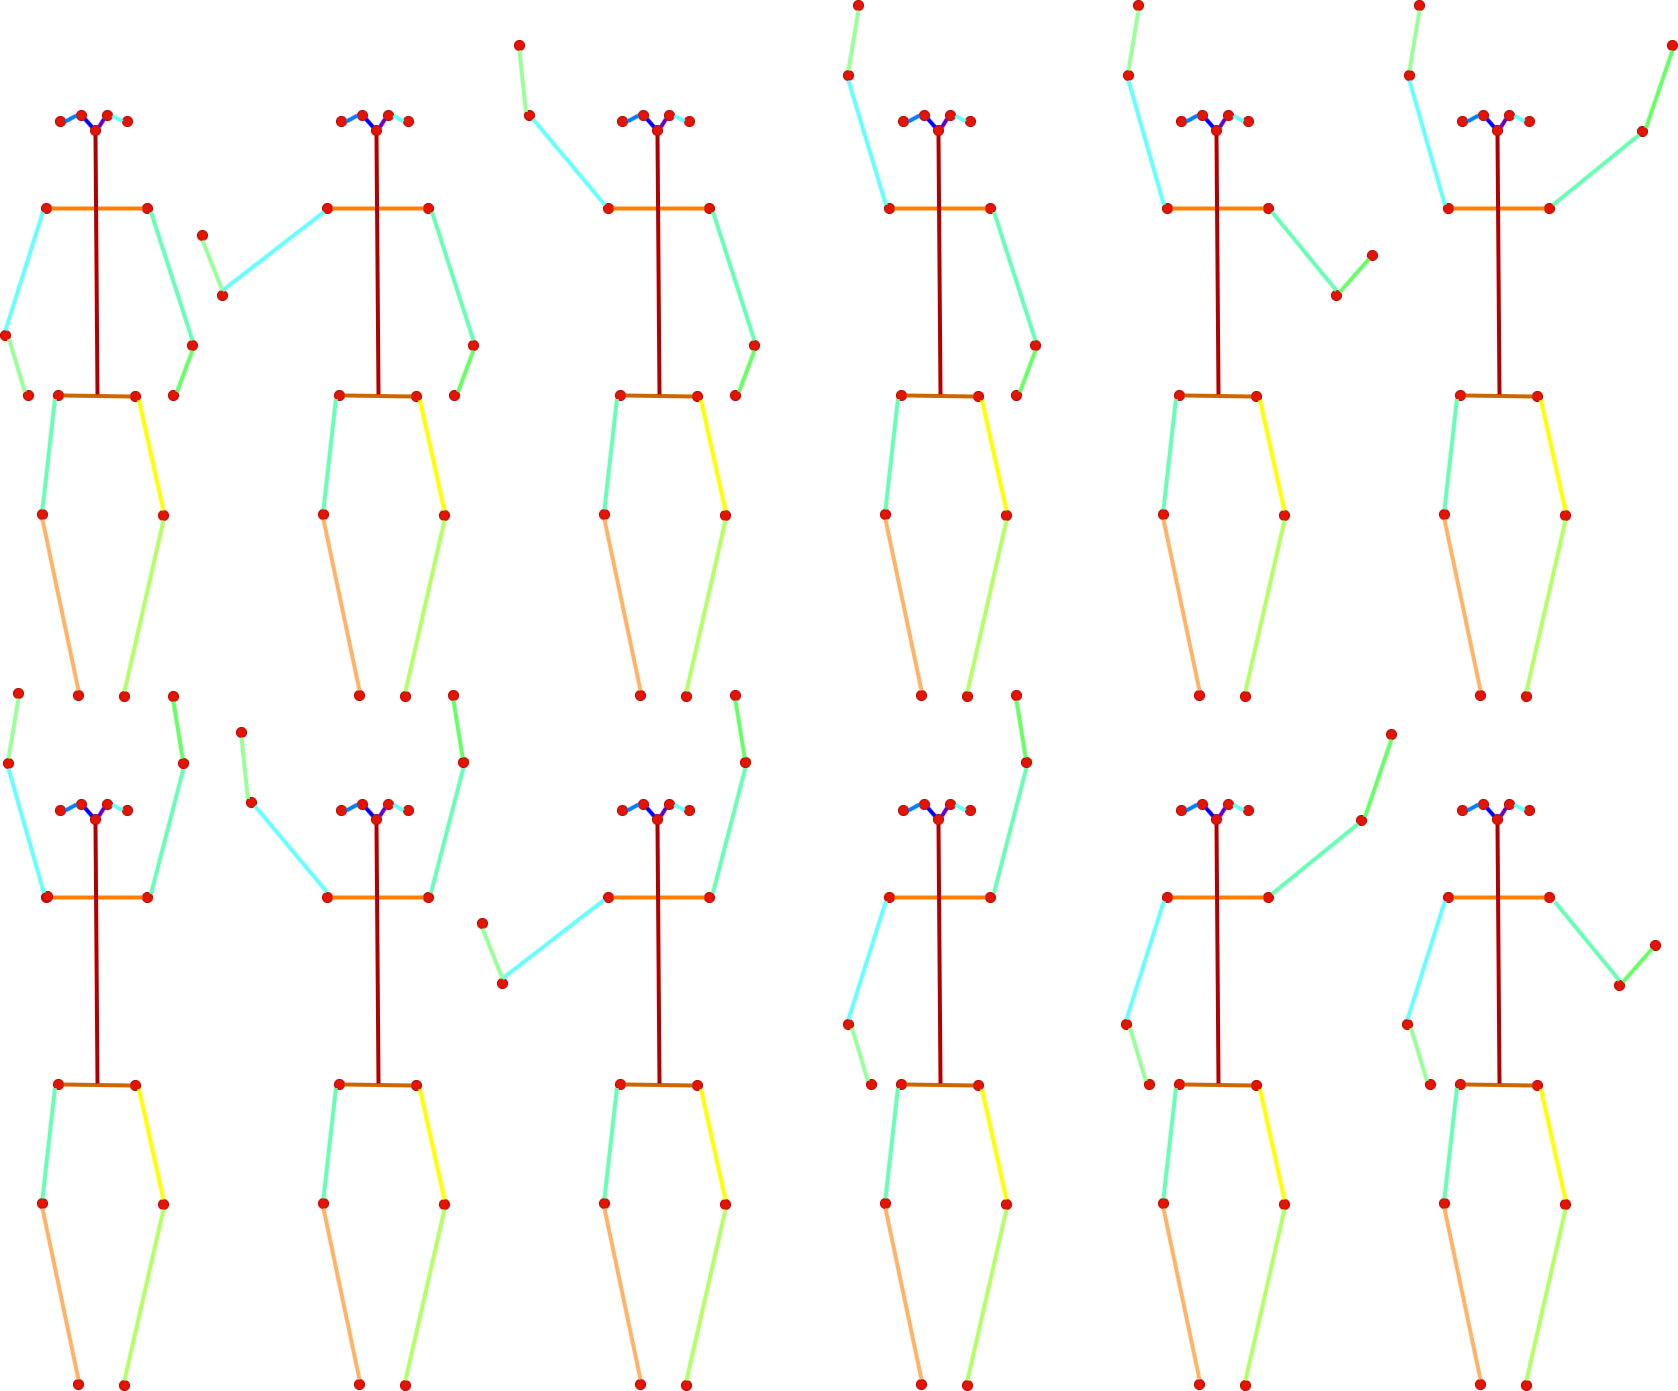
\includegraphics[width=0.75\textwidth]{plantillaLatex-master/img/skeleton3.png}
    %Skeletons_Black.png}
    \caption{Secuencia de movimientos de las extremidades superiores.}
    \label{f:f_esq_}
\end{figure}

El algoritmo que se ha creado para la detección de secuencias tiene en cuenta estas problemáticas. Por otra parte otro problema a tener en cuenta es el tipo de ejercicios. A simple vista para un individuo es muy sencillo diferenciar entre un movimiento de brazos horizontal o vertical pero esto sumado a los inconvenientes anteriormente nombrados hace que para el algoritmo no lo sea tanto. 

Imaginémonos que tenemos a un terapeuta que realiza múltiples ejercicios para sus pacientes. Entre los ejercicios que realiza, varios de ellos ejecutan las extremidades superiores del cuerpo. Nuevamente hay que tener en cuenta que este algoritmo está diseñado para pacientes con la enfermedad del \textit{Parkinson} por lo que los ejercicios serán cortos y varios de ellos similares. Uno de los ejercicios será mover horizontalmente los brazos y otro ejercicio será moverlos verticalmente. El paciente realiza ambos ejercicios pero en uno de ellos, por las razones que sea, ejecuta varios movimientos en las extremidades inferiores.

Una vez acabados los vídeos del paciente se procede a analizarlos. El terapeuta quiere comprobar como de bien se ha realizado el movimiento vertical de brazos. Al analizar ambos ejercicios el programa se da cuenta de que tiene por una parte, unos datos de posiciones inferiores muy parecido al del terapeuta pero las posiciones superiores no lo son tanto, y por otra parte pasa al contrario, tiene uno en que las posiciones superiores son más parecidas a las de referencia pero las inferiores no. ¿Qué secuencia seleccionará el programa como posible solución?

Este ha sido el mayor problema al que se ha enfrentado el algoritmo y es por ello que se ha propuesto en líneas futuras, ver apartado \ref{cap:linFutu}, realizar la búsqueda de secuencias una vez se tenga clasificado el ejercicio. De esta manera se le pueden otorgar diferentes pesos a las extremidades en movimiento para poder localizarlas de una forma más precisa en la secuencia compuesta por todos los ejercicios. 

Esta métrica no se ha implementado en el proyecto ya que la clasificación de ejercicios según las extremidades en movimiento se realizó posterior a la localización de secuencias como un extra, y es simplemente un posible planteamiento de como se podría implementar, por lo que aun no es una métrica del todo fiable.


\section{Soluciones al problema}

En este apartado se detallarán las diferentes lineas de actuación planteadas que se han llevado a cabo para la detección de un algoritmo que funcione con una amplia cantidad de casos, sus inconvenientes y cuales han sido las posibles soluciones o porque han sido descartadas definitivamente. Sobre el algoritmo utilizado se han tenido en cuenta varios aspectos.

El primero de ellos ha sido el tratamiento de los valores nulos. Todos los vídeos que se han procesado, son vídeos idóneos para obtener un buen resultado ya que en ellos aparece un único individuo y en todo momento se pueden apreciar la figura completa del esqueleto. Aún así, en ocasiones \textit{Detectron2} no ha extraído correctamente los esqueletos y ha generado algún valor nulo. Eliminar este tipo de valores es algo demasiado imprescindible para el correcto funcionamiento de nuestro código. 

En caso de contar con valores nulos en la secuencia que comprende el conjunto completo de ejercicios, el algoritmo detecta esos valores como el camino más óptimo y devuelve como \textit{frame} de inicio y final del ejercicio de referencia el correspondiente a la posición en la que se han localizado los valores nulos. Es decir, si tenemos una secuencia de longitud $N$ que contiene un valor nulo en la posición $k$ siempre que $k \in N$, localizará $k$ como instante de inicio del ejercicio y ese mismo $k$ como instante final.

Para evitar esta búsqueda errónea de ejercicios se ha procesado a buscar y eliminar todos los nulos en el instante previo al análisis. Estos valores podrían haber sido sustituidos por una media de los valores próximos pero en una ejecución que generaba 1294 objetos de tipo esqueleto, contando con que cada objeto está compuesto por 27 posiciones y cada posición por sus coordenadas en el eje $X$ y en el eje $Y$, haciendo un total de 69.876 valores, contando los ceros almacenados en el eje $Y$ de los ángulos, solo se obtuvieron dos valores nulos, por lo que la eliminación de los mismos no parece que vaya a tener mucha repercusión en el correcto funcionamiento del programa. 

Otro problema con el que hubo que lidiar fue con la mala obtención del camino óptimo en las pruebas con datos multidimensionales. En las pruebas con datos multidimensionales al contar con datos tan amplios y muchas veces demasiado dispersos entre ellos el algoritmo funcionaba de una manera muy poco precisa. 

Finalmente, como se comentaba con anterioridad en el apartado \ref{cap:defProblem}, el problema principal de este proyecto ha sido la localización de secuencias completas independientemente de su longitud. Esto con la alineación \textbf{DTW} parecía estar solucionado pero en ciertas ocasiones no ha sido así. Para explicar el porque de este problema vamos a plantear un ejemplo. 

Si contamos con las siguientes secuencias:
\begin{enumerate}
    \item - Patrón de referencia, [[10,4,45,6],[34,67,2,56],[34,56,78]]
    \item - Secuencia en la que buscar, [[564,444,435,2346],[3344,6347,32,5634], [33244,5346,7438],[10,400,465,6], [3454,6547,52,556],\textbf{[60,40,80]}, [10234,3424,435,634]]
\end{enumerate}

Como se puede observar el patrón de referencia es una matriz compuesta por tres filas y la matriz en la que se pretende buscar dichos valores tiene un total de siete filas, ambas tienen idéntico número de columnas. Lo que el algoritmo de \textbf{DTW} realiza para la búsqueda de secuencias es observar el patrón y buscar una similitud dentro de la cadena larga pero, como solo encuentra similitud con una parte del patrón, \textbf{[60,40,80]}, es esa la que devuelve.
Esto es lo que pasa en la búsqueda de secuencias de algunos de nuestro ejemplos. Como el algoritmo no encuentra coincidencias bastante favorables con el patrón, simplemente las descarta y devuelve una secuencia de una tamaño mucho menor al esperado. En la figura \ref{fig:ErrorAngles} se puede observar un ejemplo de lo comentado con anterioridad. 

\begin{figure}[H]
    \centering
    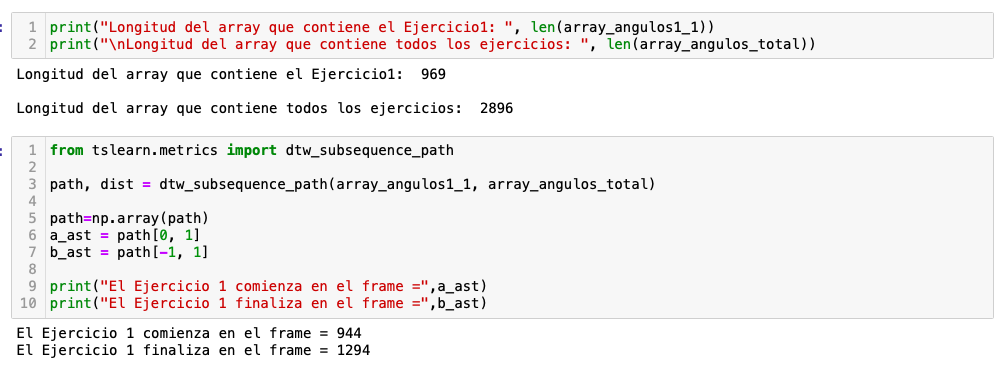
\includegraphics[width=\textwidth]{plantillaLatex-master/img/ErrorAngles.png}
    \caption{Resultado desfavorable en la localización de secuencias.}
    \label{fig:ErrorAngles}
\end{figure}

Para solucionar este problema se añadirá una tasa de error sobre las posiciones localizadas. De esta manera añadirá unas posiciones extras al comienzo y al final del ejercicio. No es la solución más óptima ya que en algunos casos hará que el ejercicio comience mucho antes de lo esperado o que no llegue a terminar, y en otros casos, cuando encuentre la secuencia prácticamente a la perfección hará que se le añada parte de otros ejercicios. 


\section{Extracción de datos}

En este apartado se va a exponer las soluciones planteadas para la extracción de las secuencias. Todo el flujo relativo al procesamiento de vídeos estaba ya implementado en el proyecto que se ha usado como punto de partida pero le faltaba la extracción de las posiciones. 

Matizar en este punto que aunque a simple vista la extracción de las posiciones parezca una operación muy sencilla, el familiarizarte con un proyecto nuevo, sobre una tecnología desconocida ha creado en algunas ocasiones múltiples quebraderos de cabeza sobre los errores arrojados.

\begin{figure}[H]
    \centering
    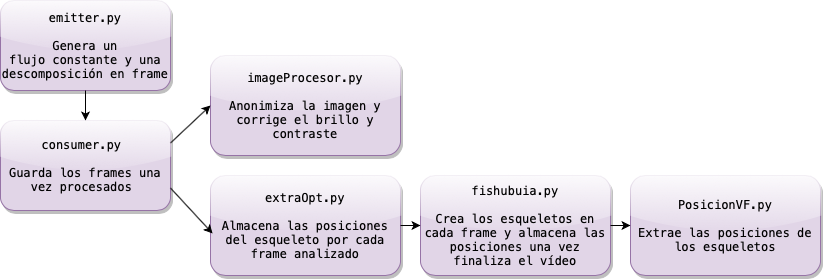
\includegraphics[width=0.9\textwidth]{plantillaLatex-master/img/Diagram_py.png}
    \caption{Estructura de ficheros.}
    \label{fig:Diagram_py}
\end{figure}

Finalmente una vez se consiguieron subsanar los problemas por los que no se conseguían almacenar las posiciones correctamente, se procedió a realizar los siguientes cambios sobre los ficheros, en la figura \ref{fig:Diagram_py} se puede observar la estructura de los ficheros y en las figuras \ref{f:ficherosModificados} y \ref{f:ficherosModificados2} los cambios realizados sobre los ficheros ya existentes:
\begin{enumerate}
    \item Fichero \textbf{emitter.py}, este fichero es el encargado de lanzar los \textit{frames} y reproducir el vídeo en bucle. Como el proyecto estaba planteado para  extraer esqueletos de pacientes en tiempo real, este fichero trata de simular un flujo que nunca termina, es por esta razón que reproduce el vídeo en bucle. Para intentar alterar lo mínimo el funcionamiento del programa, se optó por no parar el vídeo en este punto si no que emitiese un \textit{frame} totalmente negro una vez que el vídeo finalizase.
    \item Fichero \textbf{PosicionVF.py}, este fichero es el encargado de calcular las posiciones bidimensionales relativas a cada punto clave del esqueleto y de la obtención de los distintos ángulos del cuerpo. En él se han creado nuevas funciones para almacenar los ángulos individualmente, los ángulos junto con el resto de posiciones y las posiciones relativas a las partes superiores e inferiores del cuerpo humano.
    \item Fichero \textbf{extraOpt.py}, este fichero será el encargado de almacenar las posiciones en cada una de las ejecuciones. 
    \item Fichero \textbf{imageProcesor.py}, finalmente este fichero se encargará de obtener las posiciones que genera el fichero \textit{PosicionVF.py} y enviarlas a \textit{extraOpt.py} para que se encargue de su almacenamiento. Este fichero también proporciona un control de errores y uno de ellos es lanzar un mensaje cuando \textit{Detectron2} no es capaz de extraer el esqueleto, es decir, cuando no encuentra posiciones. Una vez ha entrado en esta excepción, si comprobamos que el \textit{frame} del que no se esta obteniendo el esqueleto es un \textit{frame} totalmente negro, quiere decir que se ha alcanzado el final y del vídeo y por tanto duplicará lo guardado en el fichero \textit{posiciones.pickle} a un nuevo fichero que guardará únicamente las posiciones desde el principio hasta el final del vídeo.
\end{enumerate}

Cabe destacar que hay veces que esta excepción no salta ya que se deshecha el \textit{frame} antes de que llegue a ser analizado. Si esto ocurre y se observa que no aparece el fichero final, lo que se puede hacer es analizar el fichero \textit{posiciones.pickle}. Como se trata de un flujo continuo, cuando el vídeo vuelva a empezar las posiciones serán las mismas por lo que lo único que se tendría que hacer es buscar si la primera posición está repetida en el fichero, si no es así quiere decir que el programa aún no ha terminado y que necesita seguir procesándose. Sin embargo si encuentra una secuencia tal cual a la primera, está claro que no es una mera coincidencia en los movimientos del paciente si no que el vídeo se está emitiendo de nuevo. A partir de ese momento se puede parar el programa y quedarnos con todas las posiciones hasta la inmediatamente anterior a la secuencia inicial nuevamente generada. 

\begin{figure}[H]
 \centering
  \subfloat[Fichero \textbf{emitter.py}]{
   \label{f:emmiter}
    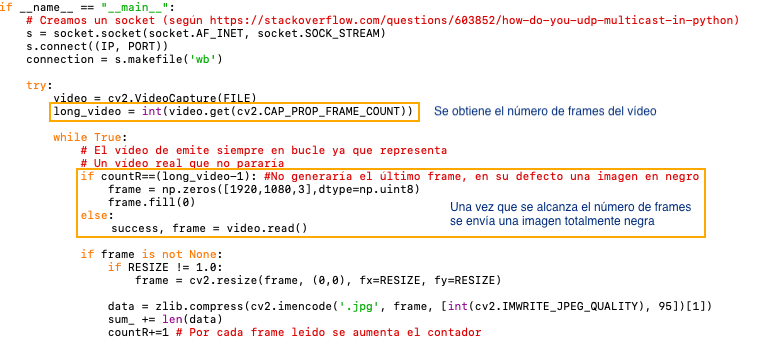
\includegraphics[width=\textwidth]{plantillaLatex-master/img/emitter.png}}\vspace{1mm}
      \subfloat[Fichero \textbf{PosicionesVF.py}]{
   \label{f:PosVF}
    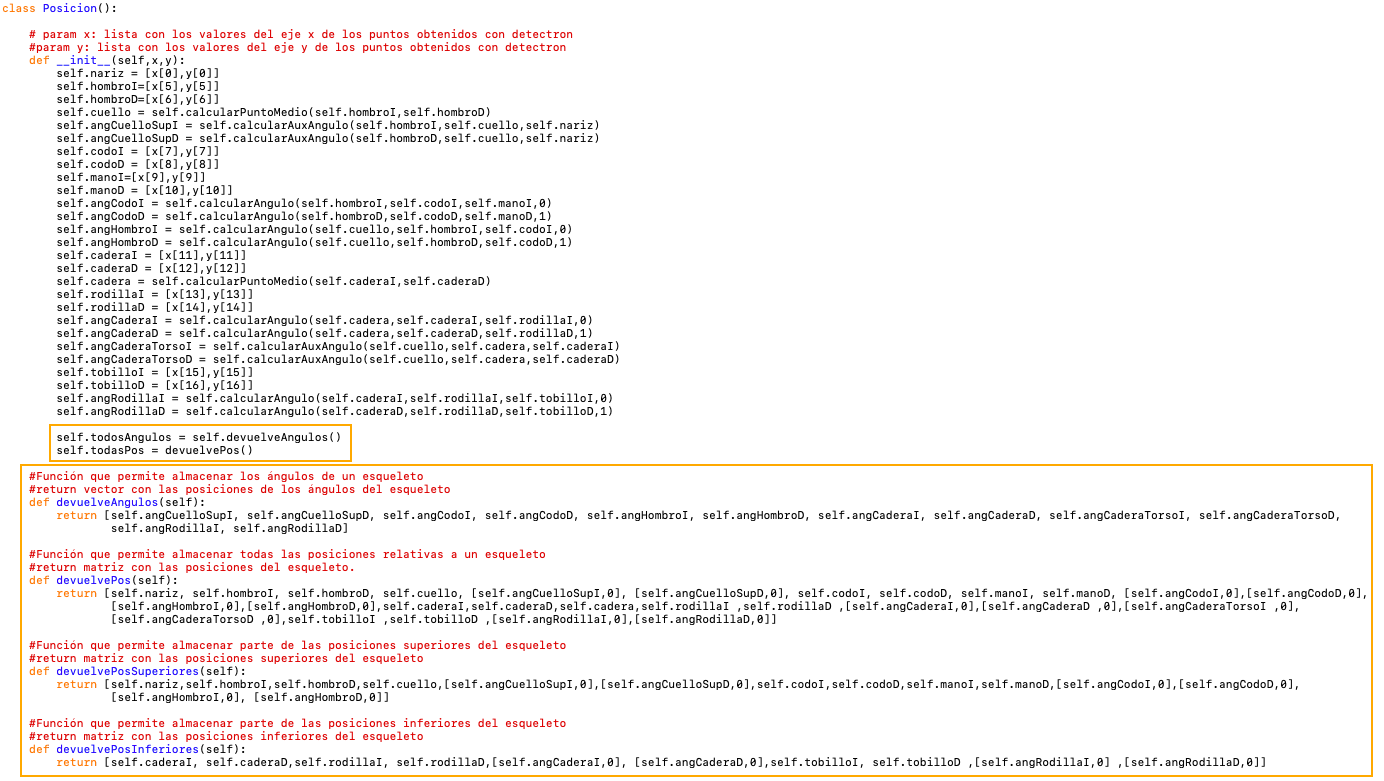
\includegraphics[width=\textwidth]{plantillaLatex-master/img/PosicionesVF.png}}
 \caption{Ficheros \textit{emitter.py} y \textit{PosicionesVF.py} modificados. }
 \label{f:ficherosModificados}
\end{figure}

\begin{figure}[H]
 \centering
  \subfloat[Fichero \textbf{extraOpt.py}]{
   \label{f:extraOpt}
    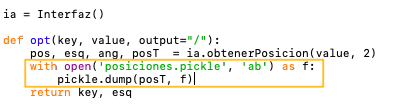
\includegraphics[width=0.8\textwidth]{plantillaLatex-master/img/extraOpt.png}}\vspace{1mm}
    \subfloat[Fichero \textbf{fishubuia.py}]{
   \label{f:fishubuia}
    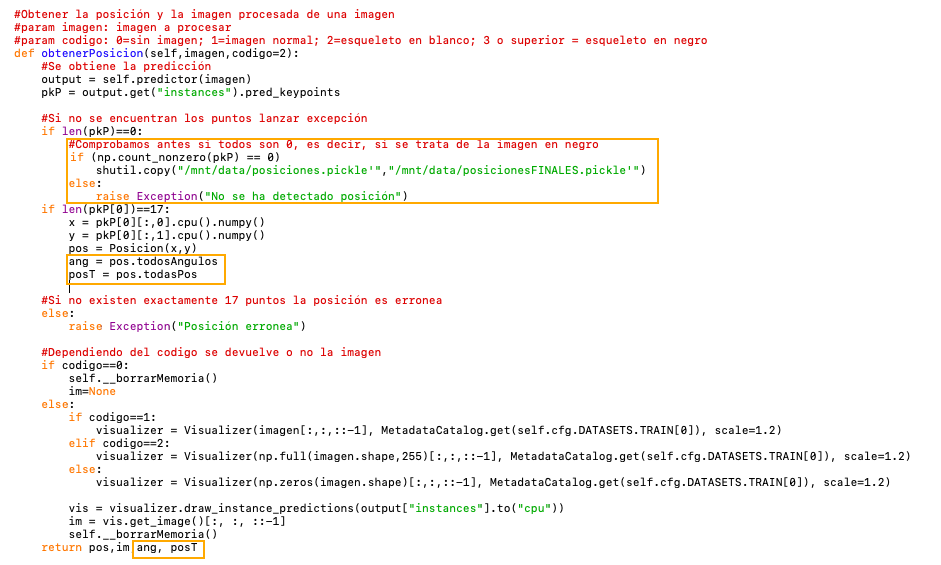
\includegraphics[width=\textwidth]{plantillaLatex-master/img/fishubuia.png}}
 \caption{Ficheros \textit{extraOpt.py} y \textit{fishubuia.py} modificados. }
 \label{f:ficherosModificados2}
\end{figure}



Otro aspecto a tener en cuenta en la extracción de las secuencias, es el tiempo que conllevan. En un sistema ideal hay que ejecutar el programa y esperar a que nos saque el total de posiciones por vídeo. En un vídeo de unos dos minutos esta acción durar alrededor de los 20 minutos, todo dependiendo de factores externos al programa como pueden ser la conexión a la red, etc. Como hemos comentado esto sucedería en un sistema ideal, pero en el apartado \textit{Manual del programador} de los anexos se exponen numeroso aspectos que comprometen el normal funcionamiento del programa. El más tedioso de ellos es la caída de contenedores. Para este proyecto se ha usado el equipo \textit{gamma} del grupo \textit{ADMIRABLE} de la Universidad de Burgos, y se ha comprobado que hay ocasiones en las que al haber más de un usuario realizando tareas sobre el mismo o por otros motivos que en ocasiones se desconoce su causa, provocan que se caiga alguno de los contenedores en ejecución lo que provoca un efecto dominó sobre el resto, abortando el correcto funcionamiento del programa. Este aspecto es clave para comprender algunas de las dificultades surgidas durante la realización del proyecto. En ocasiones era prácticamente imposible acabar correctamente una ejecución lo que demoraba el análisis de las secuencias al no poder ser obtenidas. 


\section{Metodología de estudio}

En este apartado se hará una mera introducción de los distintos planteamientos y fases que se han llevado a cabo a lo largo del proyecto. Para poder contrastar muchos de los aspectos que se van a comentar a lo largo de las secciones es recomendable revisar los \textit{notebooks} ubicados en el directorio \textbf{src/pruebas}. 

La \textbf{primera fase} comprende el estudio de las diferentes librerías aportadas en la sección \ref{cap:librerias}. De todas las librerías localizadas sólo algunas fueron útiles para la detección de secuencias. Y es que antes de probarlas sobre datos reales, debían de arrojar buenos resultados sobre datos ficticios, ya que si en secuencias de tamaños relativamente pequeños no se obtenían buenos resultados, en secuencias de mayor tamaño iban a ser desastrosos. Finalmente, para concluir esta fase, se realizaron numerosos ejemplos de como la librería escogida es capaz de encontrar no una secuencia igual, si no una secuencia lo más parecida posible al patrón de referencia. Estos ejemplos se pueden observar en el \textit{notebook} \textbf{C3\_Búsqueda\_y\_agrupación\_de\_secuencias\_SIMILARES.ipynb}.

Tras seleccionar la librería a utilizar en el proyecto, la \textbf{segunda fase} consistió en analizar la posibilidad de almacenar no una, si no varias rutas óptimas. La razón por la que se planteó esta opción es la siguiente. Como ya se ha comentado anteriormente, la búsqueda de una secuencia completa crea una deficiencia en el longitud de la secuencia esperada. Por ende, un planteamiento que podía resultar interesante es el siguiente. A partir de una secuencia, se sacan las posiciones relativas al inicio y al final de dicha secuencia, con estas posiciones calculamos por separado todas las rutas óptimas del inicio y el final dentro de la secuencia de mayor tamaño, es decir, buscamos todos los posibles inicio y finales. Hasta este momento se tienen almacenadas una serie de posiciones de donde puede empezar el ejercicio concreto dentro de la secuencia larga y donde puede finalizar. Con esa cantidad de posiciones se efectuó un análisis y se obtuvieron los resultados que se comentarán en la sección \ref{cap:segundaF}.

\begin{figure}
    \centering
    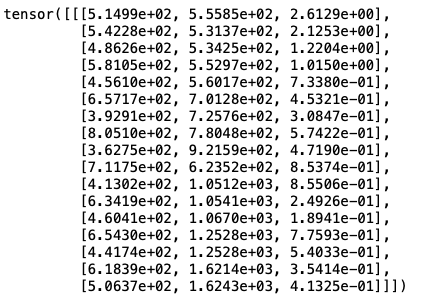
\includegraphics[width=8cm]{plantillaLatex-master/img/tensor.png}
    \caption{Datos obtenidos del fichero \textit{fishubuia.py}.}
    \label{fig:tensor}
\end{figure}

Una vez elegida la librería a utilizar para el análisis de la secuencia y la primera métrica de prueba que fue la de intentar encontrar la secuencia al completo, se decidió probar con datos reales. Inicialmente se hizo uso del elemento \emph{Posicion} que genera el fichero \textit{fishubuia.py} a partir de las posiciones extraídas mediante el fichero \textit{PosicionVF.py}. Por cada posición localizada genera unos datos como los mostrados en la figura \ref{fig:tensor}. Tras varias pruebas sobre distinto tipo de algoritmos fue descartada por varias razones:
\begin{enumerate}
    \item Al contar con tres dimensiones generaba una cantidad excesiva de datos.
    \item Las ejecuciones consumían una cantidad de tiempo inviable. Para detectar un ejercicio de una duración de 32s dentro de un vídeo completo de 1:37s, las ejecuciones sobrepasaban los 50, 60 minutos de análisis. 
    \item Por si fueran pocas las razones para no utilizar este tipo de datos, los resultados obtenidos estaban lejos de los esperados.
\end{enumerate}

Tras comprobar que este tipo de datos no fueron para nada los esperados comenzó la \textbf{tercera fase}. En esta fase se obtuvieron los datos completos a partir de los métodos creados en el fichero \textit{PosicionVF.py}. A partir de dichos datos se procedió a implementar  la búsqueda de varios posibles inicios y finales de ejercicios concretos dentro de la secuencia de mayor tamaño. Y además se usó el mismo procedimiento en la \textbf{cuarta fase} para localizar la secuencia central del ejercicio.

Finalmente y tras ver que los resultados obtenidos estaban demasiado lejos de los esperados, se puso comienzo a la \textbf{quinta fase}. En esta fase se extrajeron dos conjuntos de datos, por una parte, se obtuvieron todos los datos relativos a los ángulos y por otra parte todo el conjunto de posiciones, que abarcaba tanto los ángulos como los puntos clave del esqueleto humano. Para ello se utilizaron las nuevas funciones, anteriormente nombradas, que contiene el fichero \textit{PosicionVF.py}. Con estos conjuntos de datos se realizaron dos análisis por separado que se pueden comprobar en los \textit{notebooks},  \textbf{C6\_Pruebas\_busqueda\_angulos.ipynb, C7\_Pruebas\_busqueda\_posiciones.ipynb} y \\ \textbf{C8\_Pruebas\_recortando\_frames.ipynb,}, todos buscaban la secuencia de ejercicios concretos dentro de la secuencia de mayor tamaño. 


\section{Primera fase: Análisis de librerías}

En el apartado \textit{Técnicas y herramientas} \ref{cap:tecHerra} se comentan a grandes rasgos muchas de las librerías analizadas para poder ser aplicadas a la búsqueda de secuencias, en concreto a la búsqueda posiciones de esqueletos. En este apartado vamos a comentar las más relevantes.

Para escoger una buena librería se han tenido en cuenta los siguientes factores:
\begin{enumerate}
    \item Debe de permitir búsquedas de secuencias unidimensionales y multidimensionales.
    \item Debe de responder correctamente con grandes volúmenes de datos.
    \item El resultado arrojado debe de ser preciso, descartando aquellos resultados que contengan demasiado ruido.
    
\end{enumerate}

Por supuesto otro aspecto a tener en cuenta es que todas las librerías a utilizar sean capaces de calcular la distancia \emph{DTW}. En esta primera fase, para identificar las secuencias se probó con la librería \textit{dtaidistance}. Esta librería permite trabajar con series temporales unidimensionales y multidimensionales pero fue descartada por la baja precisión con la que se obtenían los resultados. En la figura \ref{fig:dtaidistance}, se puede observar claramente la razón por la cual no se llegó a utilizar, y es porque localiza la secuencia con demasiado ruido, no encuentra únicamente el patrón de referencia si no que lo encuentra dentro de cadenas con un tamaño demasiado elevado.

\begin{figure}
    \centering
    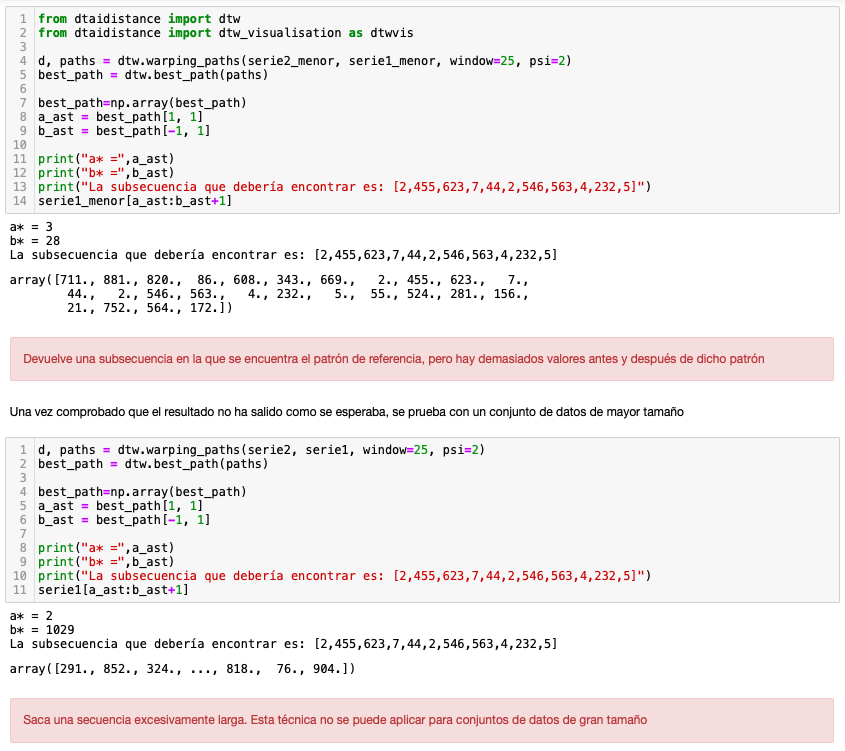
\includegraphics[width=\textwidth]{plantillaLatex-master/img/dtaidistance.png}
    \caption{Ejemplo de uso de la librería \textit{dtaidistance}.}
    \label{fig:dtaidistance}
\end{figure}

Seguidamente se probó con la librería \textbf{tslearn}. Como se puede observar en la figura \ref{f:tslearn}, esta librería es capaz de hallar una secuencia similar al patrón de referencia, devolver la posición en la que ha sido encontrada e informar sobre el grado de similitud que tiene la secuencia encontrada respecto del patrón de referencia. 

\begin{figure}
 \centering
  \subfloat{
   \label{f:tslearn1}
    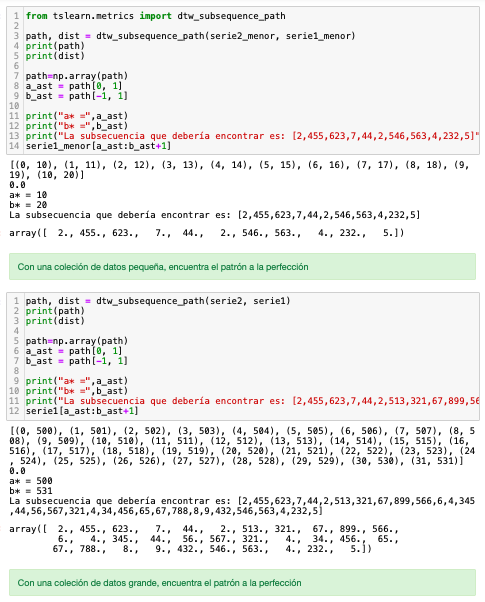
\includegraphics[width=0.9\textwidth]{plantillaLatex-master/img/tslearn1.png}}\vspace{1mm}
  \subfloat{
   \label{f:tslearn2}
    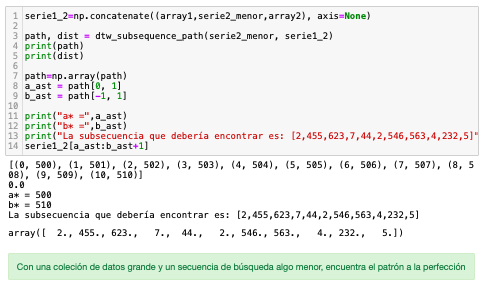
\includegraphics[width=0.9\textwidth]{plantillaLatex-master/img/tslearn2.png}}
 \caption{Ejemplo de uso de la librería \textit{tslearn}}
 \label{f:tslearn}
\end{figure}

Para constatar que se podía aplicar esta biblioteca al problema planteado se crearon diversos ejemplos con series de datos unidimensionales y multidimensionales y se observó que en todas las ocasiones arroja los resultados deseados.

Una característica a tener en cuenta que más tarde será utilizada es que, aunque la librería funcione tanto con datos unidimensionales como multidimensionales, al hacerlo con estos segundos, y sobretodo con grandes conjuntos de datos, las ejecuciones consumen una gran cantidad de tiempo. 

\subsection{Obtención de las secuencias con \textit{tslearn}}

Con la función \textbf{dtw\_subsequence\_path} de la librería \textbf{tslearn} se calcula la medida de similitud mediante \textit{DTW} entre una secuencia de referencia y otra secuencia de mayor tamaño. No es necesario que las secuencias tengan el mismo tamaño pero si que es imprescindible que tengan la misma dimensión.

\[\textbf{tslearn.metrics.dtw\_subsequence\_path(subseq, longseq)}\]

Parámetros de entrada:
\begin{enumerate}
    \item \emph{subseq}, serie temporal que representará el patrón que se desea encontrar.
    \item \emph{longseq}, serie temporal de mayor tamaño en la que se analizará donde se encuentra la secuencia más parecida al patrón de referencia.
\end{enumerate}

Parámetros de salida:
\begin{enumerate}
    \item Lista de pares enteros, ruta por la cual se puede encontrar la secuencia de referencia dentro de la secuencia de mayor tamaño. La lista está representada por pares de índices en los que la primera posición de cada tupla corresponden al elemento de \textit{subseq} y el segundo elemento de la tupla a \textit{longseq}.
    \item \textit{float}, puntuación de similitud.
\end{enumerate}

En la figura \ref{fig:dtw_subsequence_path} se puede observar un ejemplo de uso de esta función. 
\begin{figure}[H]
    \centering
    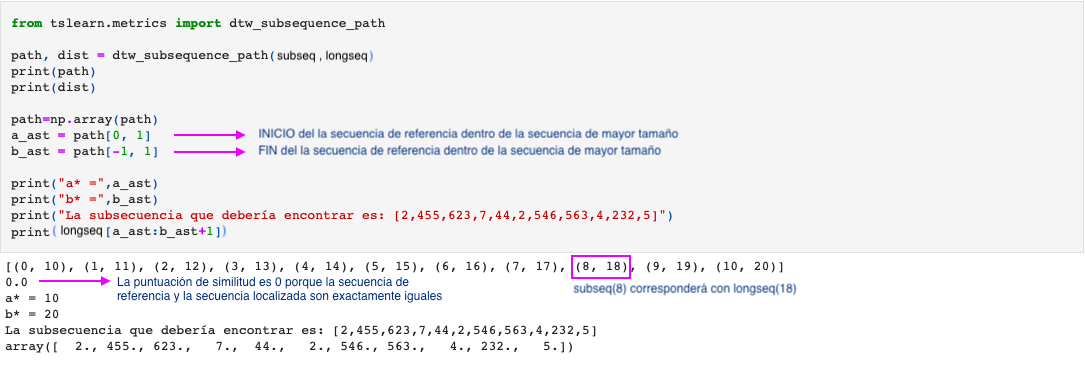
\includegraphics[width=\textwidth]{plantillaLatex-master/img/dtw_subsequence_path.png}
    \caption{ Ejemplo de uso de la función \textit{dtw\_subsequence\_path}.}
    \label{fig:dtw_subsequence_path}
\end{figure}

Finalmente matizar que el algoritmo utilizado con \textbf{tslearn} funciona tanto para valores unidimensionales como multidimensionales. En el proyecto se han realizado distintas pruebas y en algunas de ellas se han redimensionado los valores haciendo que posean una única dimensión. Esto se ha realizado por la eficiencia con la que se obtenían los resultados.


\section{Segunda fase: Búsqueda de varias secuencias} \label{cap:segundaF}

Una vez expuesto el proceso por el cual se encuentra una secuencia dentro de otra de mayor tamaño lo más parecida posible a un patrón de referencia, ahora se va a exponer como poder almacenar varias secuencias parecidas al patrón de referencia. 

Esta motivación surge de la idea de localizar múltiples secuencias para posteriormente ser analizadas y almacenar la mejor, es decir, la más parecida al patrón de referencia. Cabe destacar que las librerías anteriormente usadas hacen este proceso automáticamente, es decir, evalúan todos los posibles caminos y devuelven el que mejor distancia \textit{DTW} arroje. Ahora se va a plantear obtener todas las secuencias y más adelante que sea el usuario sea el que seleccione los criterios de clasificación que mejor le convengan para obtener la secuencia deseada.

Para poder observar ejemplos de como obtener dichas secuencias se han creado un par de \textit{notebooks}, \textbf{C4\_Búsqueda\_multiples\_secuencias} y \textbf{C3\_Búsqueda\_y\_agrupación\_de\_secuencias\_SIMILARES}. En ellos se puede observar como una vez extraídas las secuencias lo primero que se realiza es calcular las matrices de coste y las posibles rutas que sirven para encontrar las secuencias más similares al patrón de referencia. Si se quiere profundizar sobre como se ha realizado el cálculo de las matrices, por favor visitar el apartado \ref{cap:DTW}.

Como se comenta en el apartado anteriormente mencionado, a la hora de calcular la matriz de costes locales o matriz de distancias, se pueden usar diversas métricas para obtener la distancia entre las dos secuencias generadas. En este proyecto, tanto esta como todas las pruebas que conlleven el cálculo manual de dicha matriz, se han realizado utilizando la distancia \emph{euclidiana}. 


\begin{figure}
    \centering
    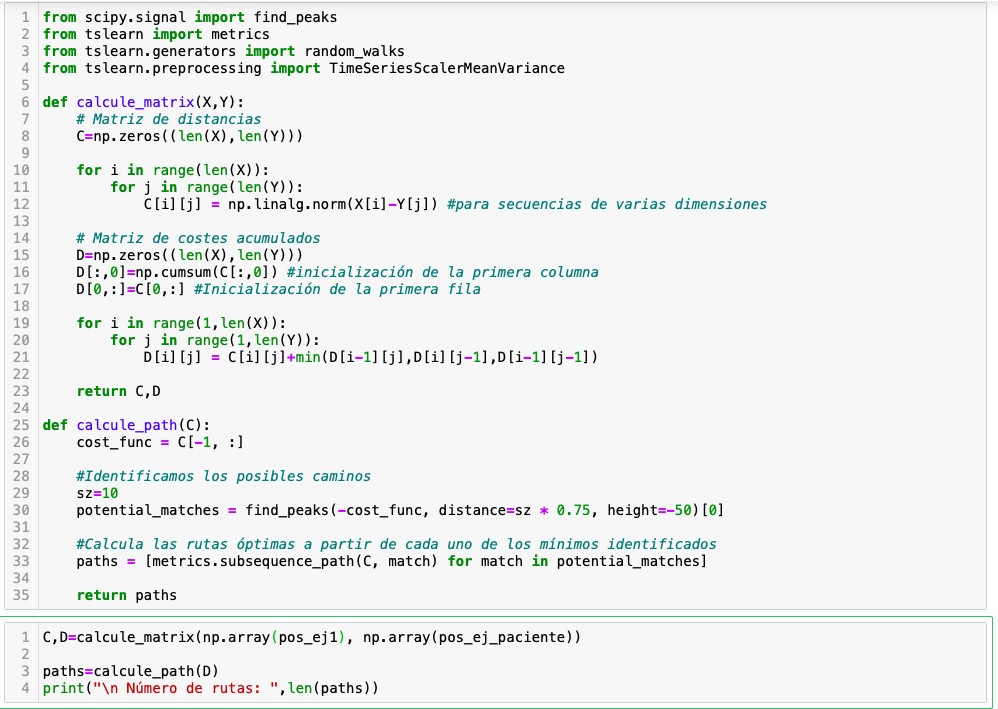
\includegraphics[width=\textwidth]{plantillaLatex-master/img/find_multiple_subsequence.png}
    \caption{Ejemplo de uso del algoritmo que localiza múltiples secuencias.}
    \label{fig:multipleSec}
\end{figure}

Por otra parte, para localizar todos las posibles rutas de deformación se ha puesto en práctica la función \textbf{scipy.signal.find\_peaks}, esta función tiene como objetivo retornar la localización de los distintos picos que se encuentran dentro de una secuencia. De esta manera podemos encontrar las secuencias similares al patrón de referencia a través de los subconjuntos de picos que se localicen en la secuencia de mayor tamaño.

En la figura \ref{fig:multipleSec} se muestra el código implementado para la búsqueda de varias secuencias. En ella se puede observar:
\begin{enumerate}
    \item \textbf{Función que calcula las matrices de coste}, en este caso las matrices no se obtendrán por medio de ninguna librería si no que serán creadas por la función \textit{calcule\_matrix(X,Y)}. Esta función recibe como parámetros dos secuencias, la primera secuencia corresponderá a la secuencia de ejercicios que se desea localizar y la segunda secuencia corresponderá al conjunto total de ejercicios realizados por el paciente en el que se desea encontrar la secuencia de menor tamaño. 
    \item \textbf{Función para calcular las posibles rutas}, como se puede observar la función \textbf{scipy.signal.find\_peaks} recibe tres argumentos. El primero hace referencia a la secuencia que contiene los picos, el segundo hace referencia a la distancia horizontal mínima. Este parámetro depende de la variable \textit{sz}, cuanto mayor sea este parámetro, mayor será la distancia entre picos y por tanto más restrictivo será el resultado obtenido. Finalmente el último parámetro que recibe la función es la altura mínima requerida para los picos. Si se hubiese recibido una secuencia con dos elementos, el primero de ellos se interpretaría como la altura mínima y el segundo como la altura máxima que podrá alcanzar el pico
\end{enumerate}

\begin{figure}[H]
    \centering
    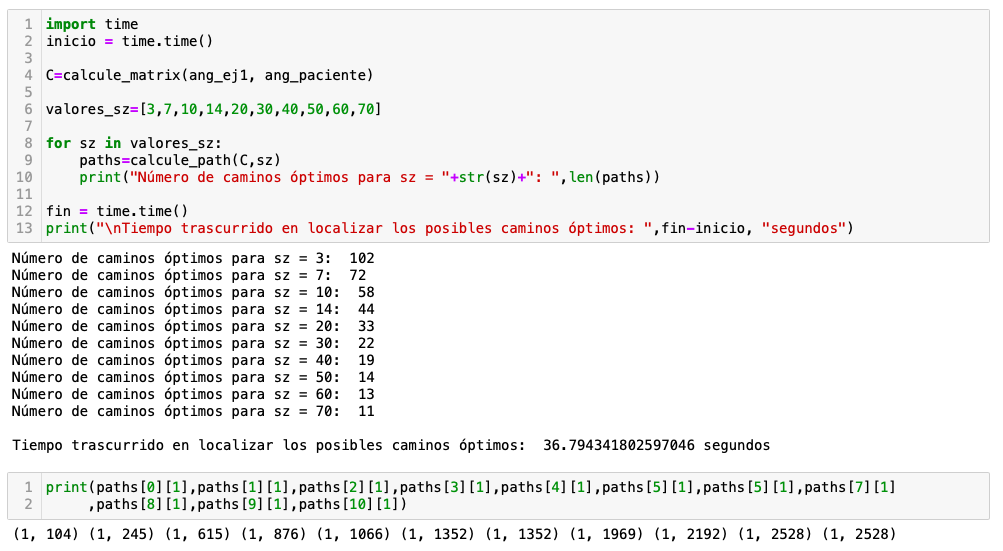
\includegraphics[width=\textwidth]{plantillaLatex-master/img/find_mult_seq_ang.png}
    \caption{Ejemplo de uso del algoritmo que localiza múltiples secuencias con ángulos.}
    \label{fig:multipleAng}
\end{figure}

Para poder observar los resultados obtenidos sobre un conjunto de datos reales, se han extraído los ángulos de un ejercicio concreto y de una secuencia de ejercicios que comprende dicho movimiento. Aunque anteriormente se ha comentado que los ángulos son datos unidimensionales, los conjuntos de datos que se analizarán tendrán múltiples dimensiones, ya que por cada \textit{frame} se extraen un total de doce ángulos. Por lo tanto, teniendo en cuenta que la secuencia del ejercicio concreto comprende un total de 969 \textit{frames} y la secuencia que contiene múltiples ejercicios comprende un total de 2896 \textit{frames}, se tendrán un patrón de referencia de dimensiones 969x12 y una secuencia larga de 2896x12. En la figura \ref{fig:multipleAng} se observan los resultados obtenidos. Cuanto mayor es el parámetro \emph{sz}, menor es el número de secuencias que encuentra, y también se puede observar como el tiempo de ejecución para la búsqueda de todos los posibles caminos con las distintas variaciones del parámetro \emph{sz}, es únicamente de 36.79 segundos, un resultado muy favorable.

Finalmente, este vídeo corresponde al vídeo \textit{Ejercicio1.mp4} que se puede encontrar en el directorio \textbf{src/pruebas/vídeos/}. Y el vídeo que comprende la secuencia de ejercicios corresponde al vídeo \textit{VideoCompleto.mp4} que se localizan en el mismo directorio. El ejercicio concreto se debería de ubicar en los 960 primeros \textit{frames} del vídeo que contiene todos los ejercicios, pero el resultado arrojado por el algoritmo, para \textit{sz=70} es el siguiente:
{\tiny \[ (1, 104) (1, 245) (1, 615) (1, 876) (1, 1066) (1, 1352) (1, 1352) (1, 1969) (1, 2192) (1, 2528) (1, 2528)\]}

Cada una de las tuplas corresponden a la posición número uno de los distintos caminos encontrados. Dentro de cada tupla, los valores se clasifican de la siguiente manera, el primer valor corresponde a la secuencia concreta y el segundo a la secuencia de mayor tamaño, es decir, para una tupla $(z,y)$ quiere decir que la posición $z$ de la secuencia de menor tamaño se encuentra alineado con la posición $y$ de la secuencia completa. Y como se puede observar en el resultado, los dos primeros valores podrían darse por válidos ya que el ejercicio debería de empezar en la posición cero, pero siempre se le dará un poco de margen o tasa de error. Sin embargo el resto de secuencias deberían de ser descartadas.


Para poder clasificar estos resultados y almacenar la secuencia que más se asimile al patón de referencia se emplearán distintas métricas de clasificación. En la tabla \ref{metricasCla} se exponen algunas de las que han sido usadas en este proyecto. Cabe destacar que todas esta métricas están seleccionadas para poder clasificar datos multidimensionales.


\begin{table}[H]
\centering
\resizebox{\textwidth}{!}{
\begin{tabular}{l}
\hline
\rowcolor[HTML]{EFEFEF} 
\multicolumn{1}{c}{\cellcolor[HTML]{EFEFEF}\textbf{Distancias DTW}}                              \\ \hline
\rowcolor[HTML]{ECF4FF} 
tslearn.metrics.dtw\_subsequence\_path(serie1, serie2)                                           \\
\rowcolor[HTML]{EFEFEF} 
dtaidistance.dtw\_ndim.distance(serie1, serie2)                                                  \\
\rowcolor[HTML]{ECF4FF} 
dtaidistance.dtw\_ndim.distance\_fast(serie1, serie2)                                            \\ \hline
\rowcolor[HTML]{EFEFEF} 
\multicolumn{1}{c}{\cellcolor[HTML]{EFEFEF}\textbf{Distancia euclidiana}}                                 \\ \hline
\rowcolor[HTML]{ECF4FF} 
dtaidistance.dtw\_ndim.ub\_euclidean(serie1, serie2)                                             \\ \hline
\rowcolor[HTML]{EFEFEF} 
\multicolumn{1}{c}{\cellcolor[HTML]{EFEFEF}\textbf{Métrica Soft-DTW}}                                     \\ \hline
\rowcolor[HTML]{ECF4FF} 
tslearn.metrics.soft\_dtw(serie1, serie2, gamma)                                                 \\ \hline
\rowcolor[HTML]{EFEFEF} 
\multicolumn{1}{c}{\cellcolor[HTML]{EFEFEF}\textbf{Coste DTW}}                                   \\ \hline
\rowcolor[HTML]{ECF4FF} 
pydtw.dtw2d(serie1, serie2)                                                                      \\
\rowcolor[HTML]{EFEFEF} 
tslearn.metrics.dtw\_path\_from\_metric(serie1, serie2)                                          \\
\rowcolor[HTML]{ECF4FF} 
tslearn.metrics.dtw(serie1, serie2, global\_constraint="sakoe\_chiba", sakoe\_chiba\_radius=0.5) \\
\rowcolor[HTML]{EFEFEF} 
tslearn.metrics.dtw(serie1, serie2, global\_constraint="itakura", itakura\_max\_slope=2.)        \\ \hline
\end{tabular}
}
\caption{Tabla con las posibles métricas de clasificación.}
\label{metricasCla}
\end{table}

En esta fase el objetivo principal fue el de almacenar varias secuencias, por lo que para obtener los resultados de la clasificación deberemos adentrarnos en la \emph{tercera fase}.


\section{Tercera fase: Búsqueda del inicio y del final}

Uno de los problemas que se obtiene con el planteamiento de buscar la secuencia al completo es la longitud de la secuencia localizada. Dicha longitud será igual o menor a la secuencia pasada como referencia y esto puede ser un inconveniente. 

Si un paciente realiza el mismo ejercicio que su terapeuta pero en un tiempo algo mayor se generarán las siguientes secuencias:
\begin{enumerate}
    \item \textbf{Secuencia $\textbf{T}$}, esta secuencia corresponderá al ejercicio que realiza el terapeuta con $T=[t_1,t_2...t_N]$ siendo $N$ la longitud de la secuencia.
    \item \textbf{Secuencia} $\textbf{P}$, esta secuencia corresponderá a los múltiples ejercicios realizados por el paciente con $P=[p_1,p_2...p_M]$ siendo $M$ la longitud de la secuencia y sabiendo que $M > N$
    \item \textbf{Secuencia} $\textbf{S}$, esta secuencia corresponderá al ejercicio que se desea encontrar dentro de la secuencia $P$ con $S=[s_1,s_2...s_K]$ siendo $K$ la longitud de la secuencia y sabiendo que $S \in P$ y que $K > N$ 
\end{enumerate}

Si el algoritmo únicamente localiza una secuencia dentro de otra de mayor tamaño, estará localizando la secuencia $S$ dentro de la secuencia $P$ con un tamaño de $N$ en vez de localizar la secuencia con su tamaño $K$. Esto producirá como resultado vídeos incompletos, que o bien acaban antes de tiempo o empiezan más tarde de lo esperado. 

Para abordar este problema se ha planteado la búsqueda de inicios y finales independientes. Para ello se han seguido los siguientes pasos:
\begin{enumerate}
    \item Obtener las $x$ primeras y últimas posiciones de cada ejercicio. Este cálculo se puede realizar mediante un porcentaje, por ejemplo el 10\% de la longitud del ejercicio, aunque en las pruebas realizadas se ha ido modificando este porcentaje para poder observar los diferentes resultados.
    \item Realizar la búsqueda de varias secuencias tanto sobre el supuesto inicio como sobre el supuesto final. De esta forma se han obtenido numerosos inicio y finales, que por supuesto dependerán de los parámetros de restricción del algoritmo, en concreto del parámetro \textit{distance} anteriormente nombrado.
    \item Enlazar cada posible inicio con cada posible final. Para poder crear una ruta de deformación lo más óptima posible, se ha enlazado la posición de inicio de cada posible secuencia de inicio con la posición de final de cada posible secuencia de final, es decir, si contamos con una ruta de inicio que comienza en el \textit{frame} 200 y finaliza en el 400, y por otra parte, dos secuencias de final que comienzan en los \textit{frames} 600, y 700 y finalizan en los 1300, 1400. Se crearán dos rutas de deformación, la primera abarcará desde el \textit{frame} 200 hasta el 1300 y la segunda desde el 200 al 1400.
    \item Una vez obtenidas todas las posibles rutas de deformación, el último paso es procesar cada una de las secuencias generadas y aplicarle ciertos criterios para que sean desechadas o aceptadas. Uno de los principales criterios de clasificación es el tamaño. Si la secuencia obtenida tiene un tamaño similar al de la secuencia de referencia con una cierta tasa de error, se aceptará como posible solución. Más adelante se aplicarán las distancias \emph{DTW} de la secuencia localizada con respecto de la secuencia de referencia. Si las distancias tienen un valor demasiado elevado quiere decir que las secuencias no se están alineando correctamente y por lo tanto que no tienen valores similares. Si por el contrario estas distancias arrojan valores bajos estará expresando que las secuencias son bastante parecidas y por tanto que se ha encontrado una secuencia óptima. 
\end{enumerate}

Una vez se conoce el proceso por el cual se empiezan a clasificar las secuencias, la duda que surge ahora es ¿cómo saber cuál es la mejor secuencia? en otras palabras, ¿cómo saber cuál es la secuencia más parecida a un patrón de referencia?.

Como se ha comentado anteriormente el tamaño es un factor clave. Muchas veces las secuencias que se obtienen son demasiado parecidas, es decir podemos tener almacenados inicios o finales consecutivos o simplemente valores demasiado cercanos. Al aplicar la unión entre los posibles inicios y los posibles finales nos pueden quedar secuencias demasiado pequeñas, o en otros casos demasiado grandes. Por ejemplo si tenemos las siguientes secuencias:
\begin{enumerate}
    \item \emph{}{secuencia-ejercicio1}, con una longitud de 50 posiciones.
    \item \emph{}{secuencia-ejercicio-completo}, con una longitud de 50 posiciones.    
    \item \emph{}{\textit{posibles\_inicios}}, [1,3,12,33,41,100].
    \item \emph{}{\textit{posibles\_finales}}, [2,35,65,150,187].
\end{enumerate}

Al juntar cada posible inicio con cada posible final, algunas de las posibles rutas que se calcularán son:
secuencia\_ejercicio\_completo[1-2], secuencia\_ejercicio\_completo[1-35], secuencia\_ejercicio\_completo[1-65],\\ secuencia\_ejercicio\_completo[1-150]. A simple vista se puede observar como la primera secuencia es demasiado pequeña y la última demasiado grande. Las otras dos secuencias no son perfectas pero son aceptables.

Es por esta razón que el primer filtro a realizar es quedarse únicamente con las secuencias que sean similares al patrón de referencia. Una vez localizadas dichas secuencias el siguiente paso será buscar el grado de similitud que tienen con respecto del patrón de referencia. Para ello se usarán las técnicas investigadas en la \textbf{segunda fase}. 

\begin{table}[H]
\centering
\resizebox{14cm}{!}{
\begin{tabular}{lllll}
\rowcolor[HTML]{EFEFEF} 
\textbf{Inicio} & \textbf{Fin} & \textbf{Distancia DTW con tsleran} & \textbf{Distancia DTW con dtaidistance} & \textbf{Coste con pydtw} \\
\rowcolor[HTML]{ECF4FF} 
49              & 229          & 2015.7734436854455                 & 2242.0713006630585                      & 3075767.82365            \\
\rowcolor[HTML]{EFEFEF} 
123             & 329          & 1974.9796179538437                 & 2277.492815798004                       & 3623770.971422           \\
\rowcolor[HTML]{ECF4FF} 
221             & 391          & 2013.5418212417126                 & 2173.8919777361834                      & 2903770.599562           \\
\rowcolor[HTML]{EFEFEF} 
245             & 420          & 2016.4642688386466                 & 2203.8221787693333                      & inf                      \\
\rowcolor[HTML]{ECF4FF} 
289             & 515          & 1967.3959282959777                 & 2378.808525040852                       & 3947960.183013           \\
\rowcolor[HTML]{EFEFEF} 
351             & 547          & 1927.2893178181143                 & 2281.1751682487525                      & 3531987.928479           \\
\rowcolor[HTML]{ECF4FF} 
396             & 572          & 1908.5767256769245                 & 2173.755612732177                       & inf                     
\end{tabular}
}
\caption{Análisis de los datos obtenidos con inicios y finales.}
\label{in_fin}
\end{table}

En la tabla \ref{in_fin} se pueden observar algunos los datos obtenidos de una ejecución en la que se han localizado un total de 16 posibles inicios óptimos y 13 posibles finales. Las diferencias de distancia y coste entre las posibles secuencias son demasiado parecidas como para poder hacer una clasificación con ellas. 

Este ha sido el problema fundamental por el que se ha descartado esta posible solución. Tras probar con múltiples librerías y funciones se llegó a la conclusión de que no se podían clasificar correctamente los ejercicios usando estas métricas por la similitud en sus resultados. 

Finalmente comentar que tras los resultados anteriormente mostrados se realizaron múltiples pruebas sobre diferentes algoritmos que calculasen distancias de otro tipo como la distancia \textit{euclidiana} o la \textit{manhattan}. Nuevamente los resultados no sirvieron para poder obtener una buena clasificación de las secuencias. 


\section{Cuarta fase: Búsqueda de una secuencia intermedia}

Esta fase surge de la misma línea de pensamiento que la fase anterior, pero en este caso lo que se planteo es buscar una secuencia que representase el punto medio del patrón de referencia. Esta idea surge por la similitud de movimientos en los inicios y finales de los ejercicios. Como posible solución se planteo la búsqueda de esta secuencia intermedia y seguidamente añadirla una cierta longitud extra tanto previa como posteriormente. 


El problema de este planteamiento fueron varios. Por una parte localizaba multitud de rutas de deformación, lo que conllevaba a múltiples secuencias intermedias. Una vez obtenidas estas secuencias, se puso nuevamente esperanza en el método de clasificación empleado en la \textbf{tercera fase}, pero los problemas acabaron siendo los mismos. Al igual que los resultados mostrados en la tabla \ref{in_fin}, en este caso tampoco se pudo realizar una buena clasificación. 


Por otra parte, aunque algunos ejercicios lograsen ser bien clasificados, el problema se encontraba al aplicar la tasa, es decir, al añadirle una longitud extra tanto por la parte inmediatamente anterior como posterior. Muchos de los ejercicios siguen un mismo patrón, por ejemplo, levantar alternativamente las manos un cierto número de veces. Si el algoritmo encontraba como camino óptimo la secuencia inicial, pensándose que es la intermedia, tras añadir a dicha secuencia las posiciones que le faltaban, creaba un ejercicio tomando parte de los anteriores. 

Tanto en esta fase como en la anterior se realizaron múltiples pruebas cambiando el tamaño de las secuencias de inicio, fin e intermedias, pero con esta técnica simplemente se obtenían un mayor número de posibles resultados y a la hora de clasificarlos surgían nuevamente los mismos problemas. 

Por estas razones estos planteamientos fueron descartados tras no obtener resultados concluyentes.

\section{Quinta fase: Búsqueda de la secuencia completa}

En esta fase se ha procedido a localizar la secuencia completa del ejercicio concreto dentro de la secuencia de mayor tamaño. Para ello esta \textbf{quinta fase} se ha dividido dos \textit{subfases}, como se puede observar en la figura \ref{fig:fase5}, por una parte se ha procedido a analizar las secuencias con datos multidimensionales, y tras ello se redimensionaron las secuencias para convertirlas en unidimensionales. En los \textit{notebooks} \textbf{C6\_Pruebas\_busqueda\_angulos.ipynb} y \textbf{C7\_Pruebas\_busqueda\_posiciones.ipynb} se pueden observar al detalle las distintas implementaciones. 

\begin{figure}[H]
    \centering
    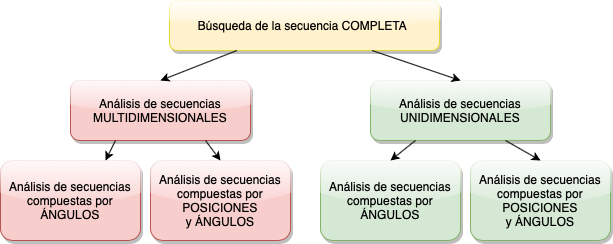
\includegraphics[width=\textwidth]{plantillaLatex-master/img/DiagramFase5.png}
    \caption{Diagrama de la quinta fase.}
    \label{fig:fase5}
\end{figure}

\subsection{Análisis de secuencias multidimensionales}

Como se ha comentado en el apartado \ref{cap:tslearn} la librería \textbf{tslearn} sirve tanto para secuencias unidimensionales como multidimensionales. Es por esta razón que será usada para todos los tipos de secuencias propuestas. 

Esta métrica de realizar las comprobaciones con secuencias multidimensionales arrojaba unos tiempos de ejecución estupendos, como se puede observar en la tabla \ref{tiempos1}. Esta tabla ha sido creada a partir de los tiempos de ejecución de cuatro secuencias compuestas únicamente por ángulos, aunque cabe destacar que con conjuntos de datos compuestos por posiciones y ángulos, los resultados son prácticamente iguales. Pero el coste de unos tiempos tan buenos son unos resultados en cuanto a la localización de secuencias nefastos. Como se puede observar en la imagen \ref{fig:angprubmulti} los resultados arrojados son excesivamente malos. Incluso después de eliminar los valores nulos, encuentra una secuencia de ejercicios con la friolera duración de dos \textit{frames}, en la que el ejercicio supuestamente comienza en la posición 1853 y termina en la posición 1856. Este tipo de resultados son totalmente inviables y tras la realización de numerosas pruebas tanto con ángulos como con la combinación de estos mismos con el resto de posiciones, se llegó a la conclusión de que trabajar con datos multidimensionales no era una opción. Aunque los tiempos de ejecución sean estupendos, no se pueden permitir unos resultados que se alejan tanto de la solución esperada. 

\begin{table}[]
\centering
\begin{tabular}{lcc}
\hline
\rowcolor[HTML]{EFEFEF} 
\multicolumn{1}{c}{\cellcolor[HTML]{EFEFEF}\textbf{Ejercicio}} & \multicolumn{1}{l}{\cellcolor[HTML]{EFEFEF}\textbf{Frames}} & \multicolumn{1}{l}{\cellcolor[HTML]{EFEFEF}\textbf{Tiempo de procesamiento}} \\ \hline
\rowcolor[HTML]{ECF4FF} 
Ejercicio 1                                                    & 969                                                         & 0.0743436 segundos                                                           \\
\rowcolor[HTML]{EFEFEF} 
Ejercicio 2                                                    & 624                                                         & 0.0438256 segundos                                                           \\
\rowcolor[HTML]{ECF4FF} 
Ejercicio 3                                                    & 626                                                         & 0.0455613 segundos                                                           \\
\rowcolor[HTML]{EFEFEF} 
Ejercicio 4                                                    & 439                                                         & 0.0343325 segundos                                                           \\ \hline
\end{tabular}
\caption{Tiempos de ejecución sobre una secuencia multidimensional larga de \textbf{2897 frames}}
\label{tiempos1}
\end{table}

\begin{figure}
    \centering
    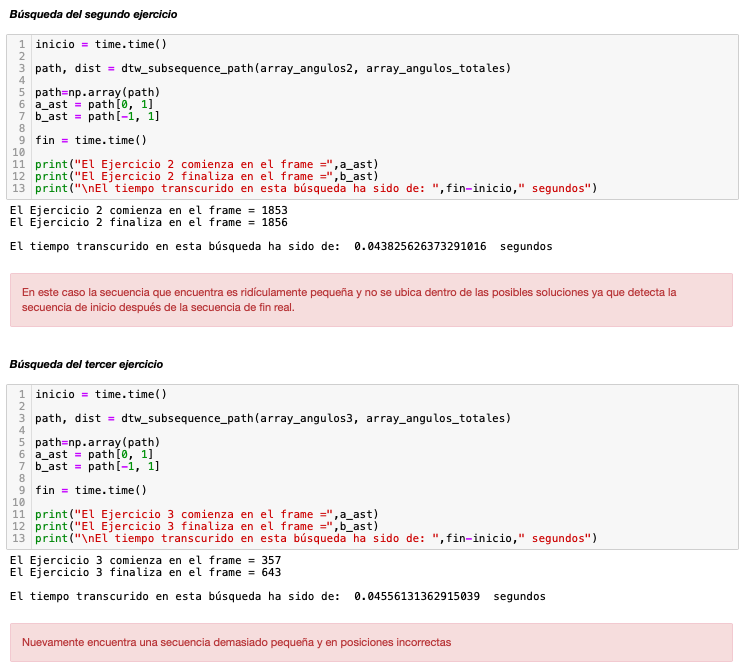
\includegraphics[width=1.2\textwidth]{plantillaLatex-master/img/find_multidimensionalts.png}
    \caption{Pruebas sobre secuencias multidimensionales compuestas por ángulos.}
    \label{fig:angprubmulti}
\end{figure}

\subsection{Análisis de secuencias unidimensionales}

Al igual que en el caso de las secuencias multidimensionales, en esta ocasión los resultados también fueron obtenidos a través del análisis que ofrece la librería \textbf{tslearn}. 

\begin{table}[H]
\centering
\begin{tabular}{lcc}
\hline
\rowcolor[HTML]{EFEFEF} 
\multicolumn{1}{c}{\cellcolor[HTML]{EFEFEF}\textbf{Ejercicio}} & \multicolumn{1}{l}{\cellcolor[HTML]{EFEFEF}\textbf{Frames}} & \multicolumn{1}{l}{\cellcolor[HTML]{EFEFEF}\textbf{Tiempo de procesamiento}} \\ \hline
\rowcolor[HTML]{ECF4FF} 
Ejercicio 1                                                    & 969                                                         & 4.927449 segundos                                                            \\
\rowcolor[HTML]{EFEFEF} 
Ejercicio 2                                                    & 624                                                         & 2.457397 segundos                                                            \\
\rowcolor[HTML]{ECF4FF} 
Ejercicio 3                                                    & 626                                                         & 2.4901232 segundos                                                           \\
\rowcolor[HTML]{EFEFEF} 
Ejercicio 4                                                    & 439                                                         & 1.7612924 segundos                                                           \\ \hline
\end{tabular}
\caption{Tiempos de ejecución sobre una secuencia unidimensional larga de \textbf{2897 frames}}
\label{tiempos2}
\end{table}


En la tabla \ref{tiempos2} se pueden observar los tiempos de ejecución de los mismos ejercicios que en la tabla \ref{tiempos1} pero en este caso las secuencias se han redimensionado a una única dimensión. Como se puede apreciar, los tiempos son algo mayores pero muy aceptables, sobretodo después de comprobar la diferencia en cuanto al resultado obtenido.

Como se puede apreciar en la figura \ref{fig:angprubuni} la secuencia correspondiente al segundo ejercicio es localizada a la perfección mientras que la correspondiente al tercero no lo es. De la misma forma y como se puede apreciar en el \textit{notebook} \textbf{C6\_Pruebas\_busqueda\_angulos.ipynb, C7\_Pruebas\_busqueda\_posiciones.ipynb} la secuencia correspondiente al cuarto ejercicio también está correctamente localizada mientras que la relativa al primer ejercicio no. Por lo tanto, hasta este punto se ha conseguido un 50\% de éxito que ya es una diferencia considerable con las técnicas anteriormente planteadas que no conseguían resultados nada favorables.

Tras comprobar que el análisis de secuencias unidimensionales con conjuntos de datos compuestos únicamente por ángulos arrojaba unos resultados bastante favorables, se probó a realizar la misma técnica pero en este caso con secuencias que almacenaban tanto los ángulos como el resto de posiciones del esqueleto. 

Como se puede comprobar en la tabla \ref{tiempos3} los tiempos de ejecución en este caso son bastante mayores, pero aún así aceptables y los resultados obtenidos fueron peores, clasificando de forma correcta únicamente el primer ejercicio. 

\begin{figure}[H]
    \centering
    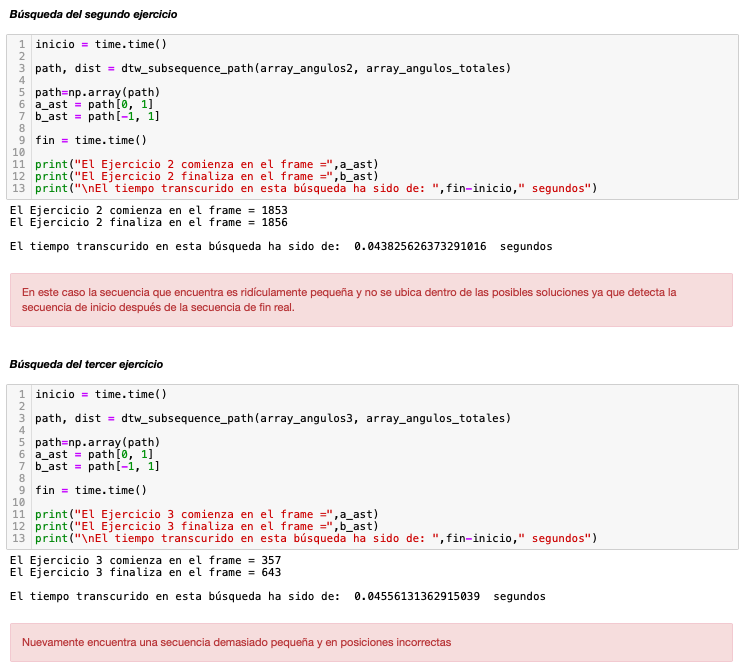
\includegraphics[width=\textwidth]{plantillaLatex-master/img/find_multidimensionalts.png}
    \caption{Pruebas sobre secuencias unidimensionales compuestas por ángulos.}
    \label{fig:angprubuni}
    
\end{figure}
\begin{table}[H]
\centering
\begin{tabular}{lcc}
\hline
\rowcolor[HTML]{EFEFEF} 
\multicolumn{1}{c}{\cellcolor[HTML]{EFEFEF}\textbf{Ejercicio}} & \multicolumn{1}{l}{\cellcolor[HTML]{EFEFEF}\textbf{Frames}} & \multicolumn{1}{l}{\cellcolor[HTML]{EFEFEF}\textbf{Tiempo de procesamiento}} \\ \hline
\rowcolor[HTML]{ECF4FF} 
Ejercicio 1                                                    & 969                                                         & 76.11154 segundos                                                            \\
\rowcolor[HTML]{EFEFEF} 
Ejercicio 2                                                    & 624                                                         & 48.85858 segundos                                                            \\
\rowcolor[HTML]{ECF4FF} 
Ejercicio 3                                                    & 626                                                         & 48.74371 segundos                                                            \\
\rowcolor[HTML]{EFEFEF} 
Ejercicio 4                                                    & 439                                                         & 34.54078 segundos                                                            \\ \hline
\end{tabular}
\caption{Tiempos de ejecución sobre una secuencia unidimensional larga de \textbf{2897 frames} compuesta por todas las posiciones y ángulos.}
\label{tiempos3}
\end{table}

Con los resultados obtenidos se decidió plantear una nueva posible solución. Los ejercicios que se pueden observar en los diferentes vídeos son ejercicios lentos que repiten un patrón, pensados para personas con la enfermedad de \textit{Parkinson}. Estas personas son, por lo general, personas mayores a las que les cuesta realizar movimientos y por lo tanto las secuencias de posiciones generadas a partir de sus vídeos comprenderán datos muy similares entre si. Es por esta razón por la que se decidió probar el análisis de las secuencias recortando algunos \textit{frames}. 

Recortando algunos \textit{frames} también se conseguiría disminuir los tiempos de ejecución y mejorar los resultados. Para poder obtener unos resultados óptimos se han realizado numerosas pruebas con distinto número de \textit{frames} pero en todas y cada una de las pruebas se seguían los siguientes pasos:
\begin{enumerate}
    \item \textbf{Redimensionar los datos}, haciendo que las dimensiones sean unidimensionales.
    \item \textbf{Eliminar los valores nulos}, para que encuentre una secuencia óptima es muy importante deshacerse de los valores nulos. 
    \item \textbf{Recortar frames}, en cada uno de las ejecuciones se iban recortando un poco más y analizando los resultados obtenidos.
    \item \textbf{Calcular su correspondencia respecto al \textit{frame} original}, para comprobar si el resultado obtenido es correcto, se debe aplicar una sencilla regla de tres y comprobar si corresponde con el \textit{frame} real. 
\end{enumerate}

Tras la creación de la aplicación de escritorio, que se comenta en el apartado \ref{cap:app}, la comprobación de resultados fue fantástica, ya que una vez obtenidos los \textit{frames} de inicio y de final, se introducen los valores en ella y se puede ver lo bien o mal que está localizando la secuencia. 

\begin{tcolorbox}
Como conclusión final a este apartado exponer que los mejores datos han sido obtenidos a partir del aproximadamente 70\% de los \textit{frames} y se pueden observar los resultados en el cuaderno \textbf{C10\_Resultados\_finales}.
\end{tcolorbox}


\section{Clasificación de ejercicios en las extremidades superiores e inferiores}

Para clasificar ejercicios según la extremidad del cuerpo que esté en movimiento se ha planteado una posible solución. Esta clasificación se consigue aplicando la desviación típica sobre el conjunto de datos obtenido. 

La desviación típica o estándar cuantifica la variación o la dispersión del conjunto de datos a analizar. Una desviación estándar baja indica que una gran parte de los datos procesados tienden a estar agrupados y a no sufrir grandes diferencias entre ellos, mientras que una desviación estándar elevada indica que los datos se extienden sobre un rango de valores bastante amplio. 

Este concepto se puede aplicar en el proyecto de la siguiente manera, si un individuo realiza movimientos sobre las extremidades superiores, éstas constantemente estarán en posiciones distintas lo que creará un conjunto de datos bastante disperso. Mientras, en ese mismo ejercicio, las extremidades inferiores estarán prácticamente inmóviles creando un conjunto de datos muy similar, es decir, un conjunto de datos muy agrupado.

Para conseguir una clasificación óptima se han probado varias técnicas:
\begin{enumerate}
    \item Probar la desviación típica sobre todo el conjunto de datos.
    \item Probar la desviación típica sobre el eje $x$ y el eje $y$.
    \item probar la desviación típica sobre distintas partes del cuerpo.
\end{enumerate}

Para ejecutar las pruebas se han separado los datos en dos conjuntos, por una parte se encuentran los valores asociados a las partes superiores del cuerpo y por otra los valores asociados a la parte inferior. Como partes superiores se entienden, nariz, hombros, cuello ángulos del cuello, codos, manos, ángulos del codo, y ángulos del hombro. Y finalmente como partes inferiores se han escogido la cadera, rodillas, ángulos tanto de la cadera como de las rodillas y los tobillos.

Con los datos separados se ha calculado la desviación estándar dos veces sobre el mismo ejercicio. Una vez sobre los datos que corresponden a las posiciones superiores del esqueleto y una segunda vez sobre los datos de las posiciones inferiores. Una vez obtenidos los dos resultados se compararán y supuestamente el que tenga mayor desviación estándar será el que indique el tipo de ejercicio que se está realizando. Se precisa de la palabra supuestamente porque a continuación se van a exponer los distintos planteamientos y las posibles soluciones que se han implementado.  

Finalmente, para comprender los ejemplos se van a exponer los ejercicios analizados en la tabla \ref{tab:ClasificacionEj1} y el tipo de movimiento que se realiza. 

\begin{table}[H]
\centering
\begin{tabular}{lc}
\hline
\rowcolor[HTML]{EFEFEF} 
\multicolumn{1}{c}{\cellcolor[HTML]{EFEFEF}\textbf{Ejercicio realizado}} & \textbf{Parte sobre la que se realiza}                              \\ \hline
\rowcolor[HTML]{ECF4FF} 
Ejercicio 1                                                              & Extremidades SUPERIORES                                             \\
\rowcolor[HTML]{EFEFEF} 
Ejercicio 2                                                              & Extremidades INFERIORES                                             \\
\rowcolor[HTML]{ECF4FF} 
Ejercicio 3                                                              & Extremidades SUPERIORES                                             \\
\rowcolor[HTML]{EFEFEF} 
Ejercicio 4                                                              & Extremidades SUPERIORES                                             \\
\rowcolor[HTML]{ECF4FF} 
Ejercicio 5                                                              & Extremidades INFERIORES                                             \\
\rowcolor[HTML]{EFEFEF} 
Ejercicio 6                                                              & Extremidades INFERIORES                                             \\
\rowcolor[HTML]{ECF4FF} 
Ejercicio 7                                                              & Extremidades INFERIORES                                             \\
\rowcolor[HTML]{EFEFEF} 
Ejercicio 8                                                              & Extremidades INFERIORES                                             \\
\rowcolor[HTML]{ECF4FF} 
Ejercicio 9                                                              & Extremidades SUPERIORES                                             \\
\rowcolor[HTML]{EFEFEF} 
Ejercicio 10                                                             & Extremidades SUPERIORES                                             \\
\rowcolor[HTML]{ECF4FF} 
Ejercicio 11                                                             & Extremidades SUPERIORES                                             \\
\rowcolor[HTML]{EFEFEF} 
Ejercicio 12                                                             & \multicolumn{1}{c}{\cellcolor[HTML]{EFEFEF}Extremidades SUPERIORES} \\
\rowcolor[HTML]{ECF4FF} 
Ejercicio 13                                                             & \multicolumn{1}{c}{\cellcolor[HTML]{ECF4FF}Extremidades SUPERIORES} \\
\rowcolor[HTML]{EFEFEF} 
Ejercicio 14                                                             & Extremidades SUPERIORES                                             \\ \hline
\end{tabular}
\caption{Clasificación de los ejercicios a analizar.}
\label{tab:ClasificacionEj1}
\end{table}


\subsection{Pruebas sobre todo el conjunto de datos}
Al probar la desviación estándar sobre todo el conjunto de datos los resultados han sido muy desalentadores. En la tabla \ref{tab:ClasificacionEj2} se muestran algunos de los datos obtenidos. 


\begin{table}[H]
\centering
\begin{tabular}{lc}
\hline
\rowcolor[HTML]{EFEFEF} 
\multicolumn{1}{c}{\cellcolor[HTML]{EFEFEF}\textbf{Ejercicio realizado}} & \multicolumn{1}{l}{\cellcolor[HTML]{EFEFEF}\textbf{Desviación típica del ejercicio}} \\ \hline
\rowcolor[HTML]{ECF4FF} 
Parte superior del Ejercicio 1                                           & 312.55                                                                               \\
\rowcolor[HTML]{EFEFEF} 
Parte inferior del Ejercicio 1                                           & 510.21                                                                               \\
\rowcolor[HTML]{ECF4FF} 
Parte superior del Ejercicio 2                                           & 317.73                                                                               \\
\rowcolor[HTML]{EFEFEF} 
Parte inferior del Ejercicio 2                                           & 478.92                                                                               \\
\rowcolor[HTML]{ECF4FF} 
Parte superior del Ejercicio 3                                           & 350.69                                                                               \\
\rowcolor[HTML]{EFEFEF} 
Parte inferior del Ejercicio 3                                           & 497.06                                                                               \\
\rowcolor[HTML]{ECF4FF} 
Parte superior del Ejercicio 4                                           & 313.89                                                                               \\
\rowcolor[HTML]{EFEFEF} 
Parte inferior del Ejercicio 4                                           & 525.45                                                                               \\
\rowcolor[HTML]{ECF4FF} 
Parte superior del Ejercicio 5                                           & 316.19                                                                               \\
\rowcolor[HTML]{EFEFEF} 
Parte inferior del Ejercicio 5                                           & 397.67                                                                               \\
\rowcolor[HTML]{ECF4FF} 
Parte superior del Ejercicio 6                                           & 295.88                                                                               \\
\rowcolor[HTML]{EFEFEF} 
Parte inferior del Ejercicio 6                                           & 463.63                                                                               \\ \hline
\end{tabular}
\caption{Desviación típica sobre cada ejercicio.}
\label{tab:ClasificacionEj2}
\end{table}

Como se puede observar, con los datos arrojados no se puede realizar ninguna clasificación. En todos los casos la desviación estándar menor se encuentra localizada en los ejercicios de la parte superior del cuerpo por lo que según los resultados presentes, todos los ejercicios deberían ser movimientos sobre las extremidades inferiores. 

Al realizar el análisis de esta manera se están juntando los valores de las dimensiones de cada posición del esqueleto, esta diferencia entre las posiciones hace que los datos sean muy dispersos. En la tabla \ref{tab:ClasificacionEj3} se muestran algunos valores que toma la cadera, tanto en el eje $X$ como en el eje $Y$.


\begin{table}[H]
\centering
\begin{tabular}{lcl}
\hline
\rowcolor[HTML]{EFEFEF} 
\multicolumn{1}{c}{\cellcolor[HTML]{EFEFEF}\textbf{Frame escogido}} & \textbf{Eje X} & \multicolumn{1}{c}{\cellcolor[HTML]{EFEFEF}\textbf{Eje Y}} \\ \hline
\rowcolor[HTML]{ECF4FF} 
Frame 1                                                             & 453.41833      & 1030.679                                                   \\
\rowcolor[HTML]{EFEFEF} 
Frame 2                                                             & 458.34384      & 1056.794                                                   \\
\rowcolor[HTML]{ECF4FF} 
Frame 3                                                             & 459.32187      & 1063.948                                                   \\
\rowcolor[HTML]{EFEFEF} 
Frame 4                                                             & 460.7943       & 1056.463                                                   \\
\rowcolor[HTML]{ECF4FF} 
Frame 5                                                             & 454.8593       & 983.5553                                                   \\
\rowcolor[HTML]{EFEFEF} 
Frame 6                                                             & 455.0474       & 1048.695                                                   \\
\rowcolor[HTML]{ECF4FF} 
Frame 7                                                             & 450.5780       & 1032.291                                                   \\
\rowcolor[HTML]{EFEFEF} 
Frame 8                                                             & 451.0298       & 1028.209                                                   \\ \hline
\end{tabular}
\caption{Valores de la desviación típica sobre la cadera.}
\label{tab:ClasificacionEj3}
\end{table}


Si se analizan por separado los valores del eje $X$ y del eje $Y$ se puede observar que están bastante agrupados pero que al juntar ambas dimensiones los valores quedan bastante dispersos. Este es un ejemplo de los ocho primeros esqueletos que está generando el algoritmo y es sólo para mostrar la dispersión entre las dimensiones. A lo largo de las ejecuciones los valores van alternándose por diferentes motivos como puede ser un cambio de postura o un movimiento involuntario. 

\subsection{Pruebas sobre el eje $X$ y el eje $Y$}

Para evitar la dispersión que genera la agrupación de dimensiones se ha optado por separarlas y calcular la desviación típica de cada ejercicio cuatro veces, se calcula las posiciones superiores en el eje $X$ y en el eje $Y$, y finalmente las posiciones inferiores se someten al mismo procedimiento. En la tabla \ref{tab:ClasificacionEj4} se pueden observar las desviaciones estándar sobre cada ejercicio y cada eje. 

\begin{table}[H]
\centering
\begin{tabular}{lcl}
\hline
\rowcolor[HTML]{EFEFEF} 
\multicolumn{1}{c}{\cellcolor[HTML]{EFEFEF}\textbf{Ejercicio realizado}} & \multicolumn{1}{l}{\cellcolor[HTML]{EFEFEF}\textbf{Eje X}} & \textbf{Eje Y}  \\ \hline
\rowcolor[HTML]{ECF4FF} 
Parte superior del Ejercicio 1                                           & 219.23                                                     & 382.54 \\
\rowcolor[HTML]{EFEFEF} 
Parte inferior del Ejercicio 1                                           & 170.64                                                     & 655.39 \\
\rowcolor[HTML]{ECF4FF} 
Parte superior del Ejercicio 2                                           & 198.50                                                     & 400.81 \\
\rowcolor[HTML]{EFEFEF} 
Parte inferior del Ejercicio 2                                           & 172.03                                                     & 616.69 \\
\rowcolor[HTML]{ECF4FF} 
Parte superior del Ejercicio 3                                           & 217.49                                                     & 441.42 \\
\rowcolor[HTML]{EFEFEF} 
Parte inferior del Ejercicio 3                                           & 163.35                                                     & 638.46 \\
\rowcolor[HTML]{ECF4FF} 
Parte superior del Ejercicio 4                                           & 205.92                                                     & 389.40 \\
\rowcolor[HTML]{EFEFEF} 
Parte inferior del Ejercicio 4                                           & 169.70                                                     & 671.78 \\
\rowcolor[HTML]{ECF4FF} 
Parte superior del Ejercicio 5                                           & 218.98                                                     & 389.03 \\
\rowcolor[HTML]{EFEFEF} 
Parte inferior del Ejercicio 5                                           & 190.47                                                     & 512.78 \\
\rowcolor[HTML]{ECF4FF} 
Parte superior del Ejercicio 6                                           & 202.11                                                     & 365.93 \\
\rowcolor[HTML]{EFEFEF} 
Parte inferior del Ejercicio 6                                           & 160.63                                                     & 600.16 \\ \hline
\end{tabular}
\caption{Desviación típica sobre todo el conjunto de datos}
\label{tab:ClasificacionEj4}
\end{table}

Nuevamente, con los datos obtenidos no se puede realizar ninguna clasificación. En el eje $X$ se obtiene una desviación típica mayor en todos los ejercicios que se realizan con la parte superior del cuerpo, mientras que en los resultados obtenidos en el eje $Y$ identifica una desviación típica mayor en los ejercicios que se realizan sobre las partes inferiores del cuerpo. Sobre ninguna de estas clasificaciones podemos sacar alguna conclusión válida. 

La razón de que fallase no es únicamente de las dimensiones. Es correcto separar las dimensiones por lo explicado anteriormente pero siguiendo en esa misma línea hay que indagar un poco más sobre los resultados. En este caso se están comparando todas las posiciones de los distintos ejes. Con todas las posiciones estamos comparando tanto rodillas, como tobillos como caderas. Esto quiere decir que aunque a lo largo de las ejecuciones no se haya apreciado prácticamente movimiento en las posiciones analizadas y la combinación de los diferentes puntos no varíe demasiado, entre ellos varía lo suficiente como para que la desviación típica arroje un resultado desfavorable. 

Al analizar la figura \ref{f:esqueletos} se puede observar que donde más varían las posiciones es a lo largo del eje $Y$, en concreto, en las partes inferiores del esqueleto, la diferencia entre la cadera y el tobillo en relación al eje $Y$ es bastante más notable que la posición del hombro respecto de las manos. Por esta razón las desviaciones típicas del eje $Y$ son bastante mayores que las del eje $X$

Con los resultados mostrados lo más preciso parece ser analizar cada punto del esqueleto.

\subsection{Pruebas sobre distintas partes del esqueleto}

Después de observar los inconvenientes que genera agrupar las distintas posiciones del esqueleto, se va a proceder a evaluar individualmente algunos de los puntos relevantes que extrae el esqueleto. En las figuras \ref{f:prub1} \ref{f:prub2} \ref{f:prub3} se muestran los resultados obtenidos tras calcular la desviación típica sobre los distintos ejes de cada ejercicio y sobre una posición concreta dentro de cada ejercicio.


\begin{figure}
 \centering
  \subfloat[Desviaciones típicas en la mano derecha.]{
   \label{f:r}
    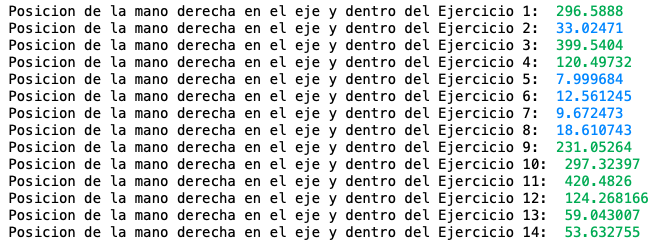
\includegraphics[width=\textwidth]{right_hand_y-axis.png}}\vspace{1mm}
  \subfloat[Desviaciones típicas en el ángulo del codo izquierdo.]{
   \label{f:r2}
    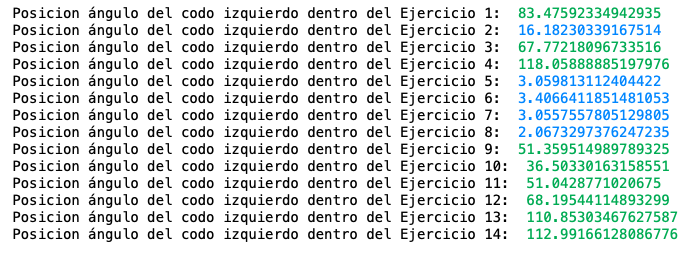
\includegraphics[width=\textwidth]{left_elbow_angle.png}}\vspace{1mm}
    \subfloat[Desviaciones típicas en el ángulo del codo derecho.]{
   \label{f:r3}
    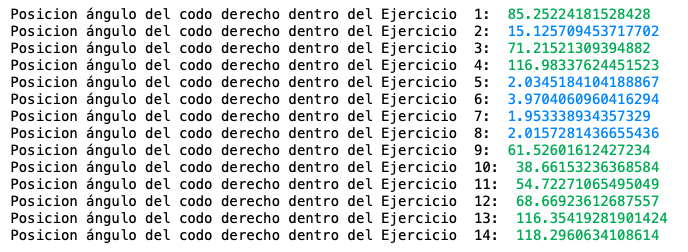
\includegraphics[width=\textwidth]{right_elbow_angle.png}}\vspace{1mm}
 \caption{Pruebas sobre diferentes desviaciones típicas.}
 \label{f:prub1}
\end{figure}

\begin{figure}
 \centering
    \subfloat[Desviaciones típicas la rodilla izquierda.]{
   \label{f:r4}
    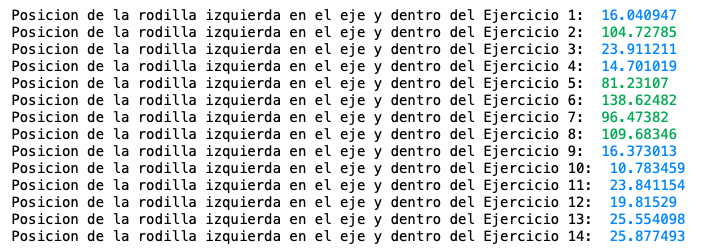
\includegraphics[width=\textwidth]{left_knee_y-axis.png}}\vspace{1mm}
      \subfloat[Desviaciones típicas en la rodilla derecha.]{
   \label{f:r6}
    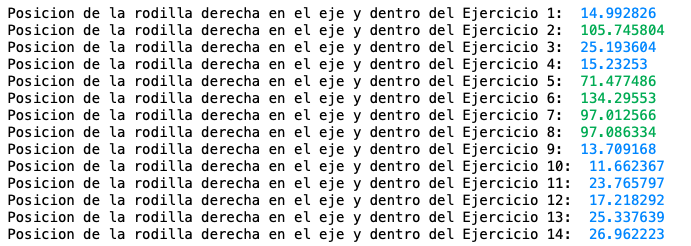
\includegraphics[width=\textwidth]{right_knee_y-axis.png}}\vspace{1mm}
      \subfloat[Desviaciones típicas en el tobillo izquierdo.]{
   \label{f:r7}
    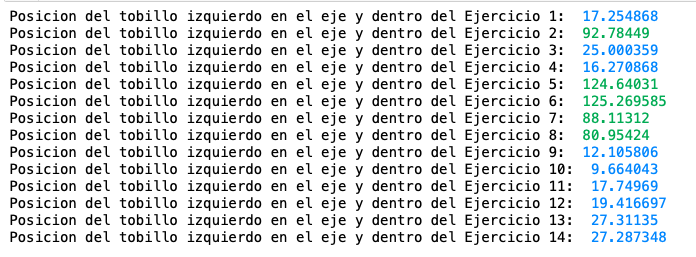
\includegraphics[width=\textwidth]{left_ankle_y-axis.png}}\vspace{1mm}
 \caption{Pruebas sobre diferentes desviaciones típicas.}
 \label{f:prub2}
\end{figure}

\begin{figure}
 \centering
\subfloat[Desviaciones típicas en el tobillo derecho.]{
   \label{f:r8}
    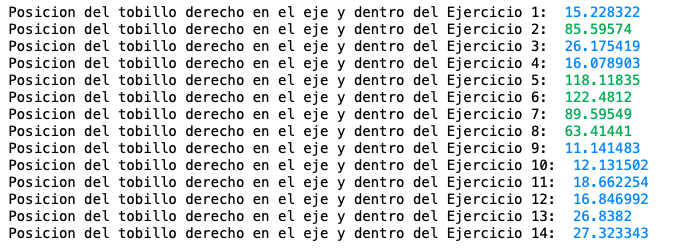
\includegraphics[width=\textwidth]{plantillaLatex-master/img/right_ankle_y-axis .png}}\vspace{1mm}
      \subfloat[Desviaciones típicas en el ángulo de la rodilla izquierda.]{
   \label{f:r9}
    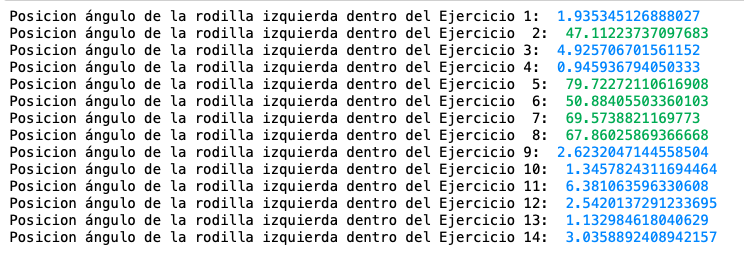
\includegraphics[width=\textwidth]{plantillaLatex-master/img/left_knee_angle.png}}\vspace{1mm}
      \subfloat[Desviaciones típicas en el ángulo de la rodilla derecha.]{
   \label{f:r10}
    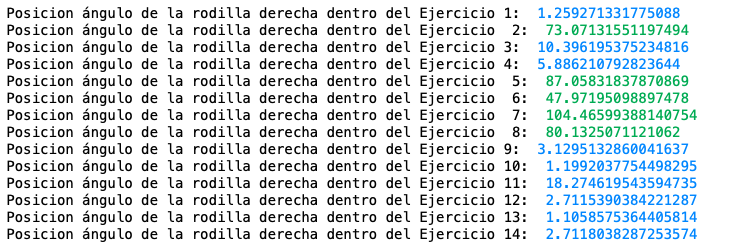
\includegraphics[width=\textwidth]{right_knee_angle.png}}
 \caption{Pruebas sobre diferentes desviaciones típicas.}
 \label{f:prub3}
\end{figure}

%left_knee_angles

Finalmente se puede concluir que con los resultados obtenidos si que se puede hacer una muy buena clasificación de si los ejercicios se realizan en la parte superior o inferior del cuerpo. Además plantearlo de esta manera es muy interesante para detectar en un futuro si el ejercicio se realiza sobre una parte más concreta del cuerpo como pueden ser movimientos de cuello.

Según los datos observados en las figuras \ref{f:prub1} \ref{f:prub2} \ref{f:prub3} las mejores clasificaciones se han obtenido en las posiciones del eje $Y$ de algunos valores, pero sin duda, los mejores resultados provienen del análisis de ciertos ángulos. 

Hay que tener en cuenta que aunque los pacientes realicen ejercicios sobre las extremidades superiores, en algún momento ejercerán un movimiento involuntario sobre alguna extremidad inferior como puede ser un cambio en la posición o un movimiento involuntario del pie. Es por esta razón que se debe intentar encontrar la mejor agrupación para el análisis de datos

\newpage
\section{Clasificación de ejercicios}

Una vez se han obtenido los valores correspondientes a las desviaciones típicas queda la parte de clasificarlas. Si se elige el ángulo de la rodilla derecha como punto de clasificación, habrá que agrupar los ejercicios que contengan una desviación típica elevada como ejercicios sobre las parte inferior del cuerpo, mientras que si cuentan con un valor bajo de desviación típica, se agruparán como ejercicios sobre la parte superior, pero ¿qué se considera un valor bajo o un valor alto?

Esta respuesta se puede responder con el concepto de deciles, cuartiles o percentiles. 
\begin{enumerate}
    \item \textbf{Cuartiles}, los cuartiles son tres valores $Q1$ $Q2$ $Q3$ que dividen el conjunto de datos y los ordenan en cuatro partes porcentualmente iguales.
    \item \textbf{Deciles}, los deciles son nueve valores que dividen el conjunto de datos en diez partes porcentualmente iguales. El primer decil $D_1$ indica que solamente existe una probabilidad del 10\% de que la variable esté por debajo de esta cifra.
    \item \textbf{Perentiles}, los percentiles son tal vez la medida más utilizada para el propósito de clasificación de características humanas. Los percentiles son 99 valores que dividen el conjunto en cien partes iguales de datos ordenados. El primer percentil $P_1$ indica que un valor supera el al uno por ciento de los valores y es superado por el noventa y nueve por ciento restante.
\end{enumerate}



Para la clasificación de los ejercicios se ha elegido la medida de \textbf{percentil}. En la tabla \ref{tab:PercentileRank} se puede observar un ejemplo de como el percentil clasifica con valores más altos los ejercicios que tienen una desviación típica mayor. De esta manera se podría lograr una clasificación de varios ejercicios.

Finalmente si lo que se espera es clasificar un único ejercicio la clasificación anterior nos es inválida ya que no se tienen otros ejercicios con los que comparar las desviaciones típicas. Lo que si que se obtiene son desviaciones típicas de distintas partes del cuerpo.

\begin{table}[H]
    \centering
    \begin{tabular}{}
    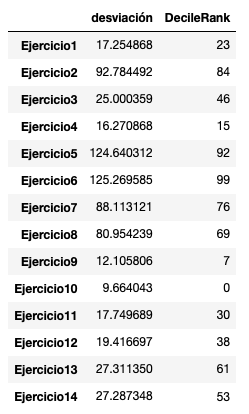
\includegraphics[width=0.32\textwidth]{PercentileRank.png}
    \end{tabular}
    \caption{Clasificación de los ejercicios según el valor del \textbf{percentil}.}
    \label{tab:PercentileRank}
\end{table}

 Para conseguir clasificar un ejercicio se pueden obtener las desviaciones típicas de partes superiores del cuerpo como las manos o los codos, y por otra parte, desviaciones típicas de las partes inferiores, como los tobillos o las rodillas. Si las desviaciones típicas de las partes superiores son mayores que las de las partes inferiores, quiere decir que se trata de un ejercicio sobre las partes superiores del cuerpo, de lo contrario sería sobre las partes inferiores. En la tabla \ref{tab:ExerciseClasification} se puede observar un ejemplo de este tipo de clasificación y en la imagen \ref{f:prub} una serie de resultados de dichas clasificaciones.

\begin{table}[H]
 \centering
  \subfloat{
   \label{f:esqueleto1}
    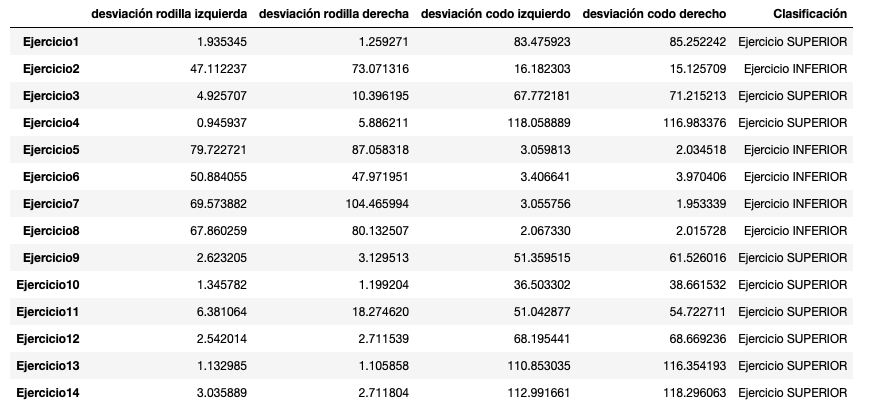
\includegraphics[width=\textwidth]{ExerciseClasification.png}}
 \caption{Clasificación teórica de ejercicios.}
 \label{tab:ExerciseClasification}
\end{table}

\begin{figure}
 \centering
\subfloat{
   \label{f:r8}
    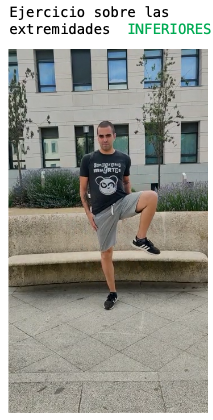
\includegraphics[width=0.25\textwidth]{plantillaLatex-master/img/ExInf4.png}}
      \subfloat{
   \label{f:r9}
    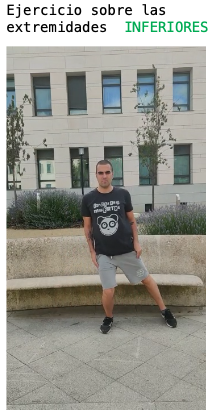
\includegraphics[width=0.25\textwidth]{plantillaLatex-master/img/ExInf3.png}}
      \subfloat{
   \label{f:r10}
    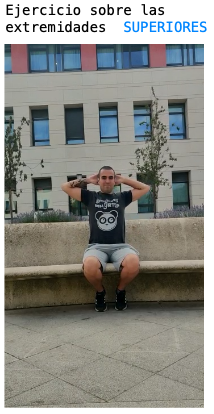
\includegraphics[width=0.25\textwidth]{plantillaLatex-master/img/ExInf2.png}}\vspace{1mm}
\subfloat{
   \label{f:r8}
    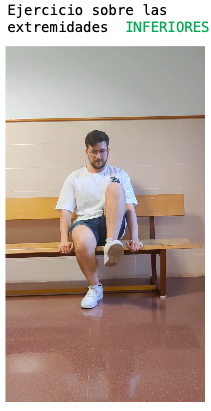
\includegraphics[width=0.25\textwidth]{plantillaLatex-master/img/ExSup4.png}}
      \subfloat{
   \label{f:r9}
    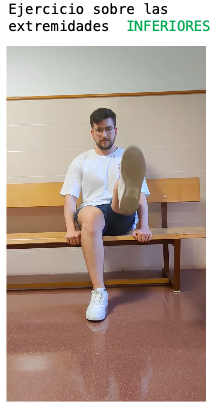
\includegraphics[width=0.25\textwidth]{plantillaLatex-master/img/ExInf1.png}}
      \subfloat{
   \label{f:r10}
    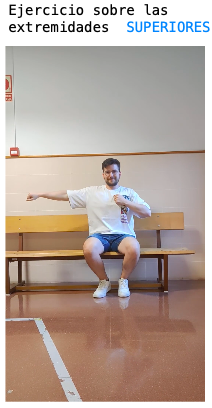
\includegraphics[width=0.25\textwidth]{plantillaLatex-master/img/ExSup3.png}}\vspace{1mm}
\subfloat{
   \label{f:r9}
    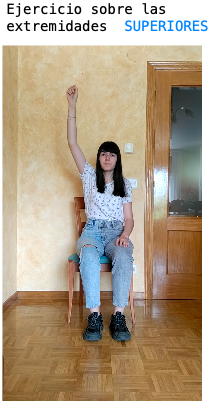
\includegraphics[width=0.25\textwidth]{plantillaLatex-master/img/ExSup2.png}}
      \subfloat{
   \label{f:r10}
    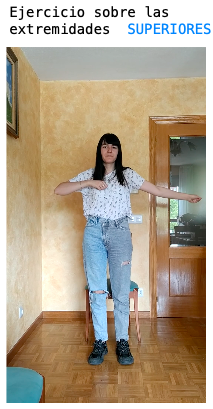
\includegraphics[width=0.25\textwidth]{plantillaLatex-master/img/ExSup1.png}}
    \subfloat{
   \label{f:r10}
    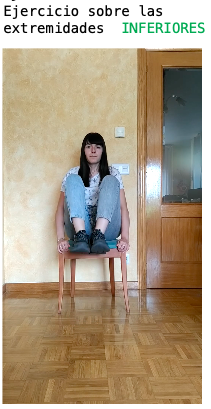
\includegraphics[width=0.25\textwidth]{plantillaLatex-master/img/ExtInf5.png}}
 \caption{Clasificación visual de ejercicios.}
 \label{f:prub}
\end{figure}
\newpage


\section{Aplicación de escritorio} \label{cap:app}

Para concluir y poder comprobar visualmente los resultados de este proyecto se ha creado una aplicación de escritorio por medio de la interfaz de \textit{Python} \textit{\textbf{Tkinter}}. Con el objetivo de poder mostrar un ejemplo más visual de las secuencias localizadas y como se podría adaptar el objetivo de este proyecto a un producto comercial. 

En esta aplicación se podrán cargar tantos vídeos como el usuario desee. Habrá una sección dedicada a los vídeos concretos, es decir, a aquellos vídeos que realiza el terapeuta, otra sección con los vídeos completos, los que realizan los pacientes, y finalmente una sección en la que se mostrará el resultado final. Todos los vídeos se podrán reproducir y pausar en la misma aplicación. 

Para ello se ha realizado una única pantalla en la que se pueden realizar las siguientes acciones:
\begin{enumerate}
    \item Al iniciar la aplicación se cargarán los vídeos de las carpetas de referencia.
    \item Los vídeos se reproducirán en la misma pantalla y cada uno en su sección correspondiente.
    \item Las funciones de recorte dependerán del modo seleccionado. Si el usuario selecciona \textit{modo ejemplo ON} los vídeos se recortarán automáticamente, mientras que si el usuario selecciona \textit{modo ejemplo OFF} se deberá de especificar los \textit{frames} de inicio y final del vídeo.
    \item Todos los vídeos se podrán reproducir y pausar.
    \item Una vez generado el recorte del vídeo, este mismo se guardará en la carpeta en la que se está ejecutando la aplicación.
\end{enumerate}

\begin{figure}
    \centering
    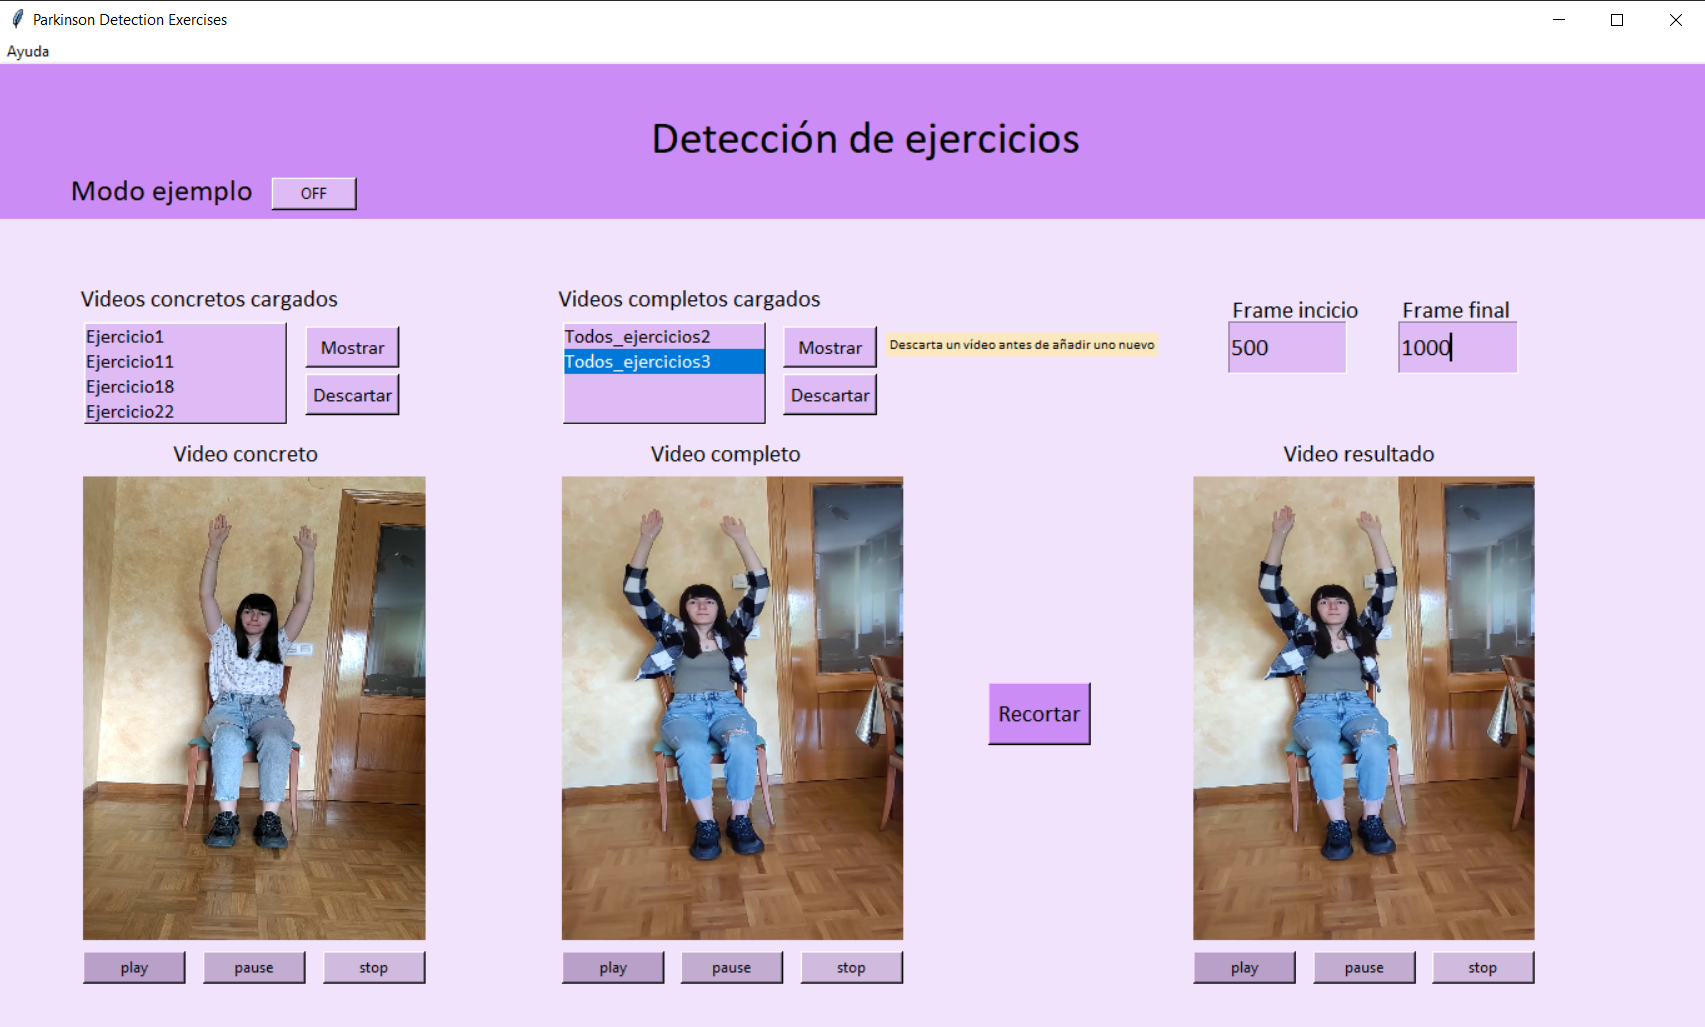
\includegraphics[width=\textwidth]{plantillaLatex-master/img/app4.PNG}
    \caption{Recorte de vídeos en modo ejemplo OFF.}
    \label{fig:app4_}
\end{figure}

\begin{figure}
    \centering
    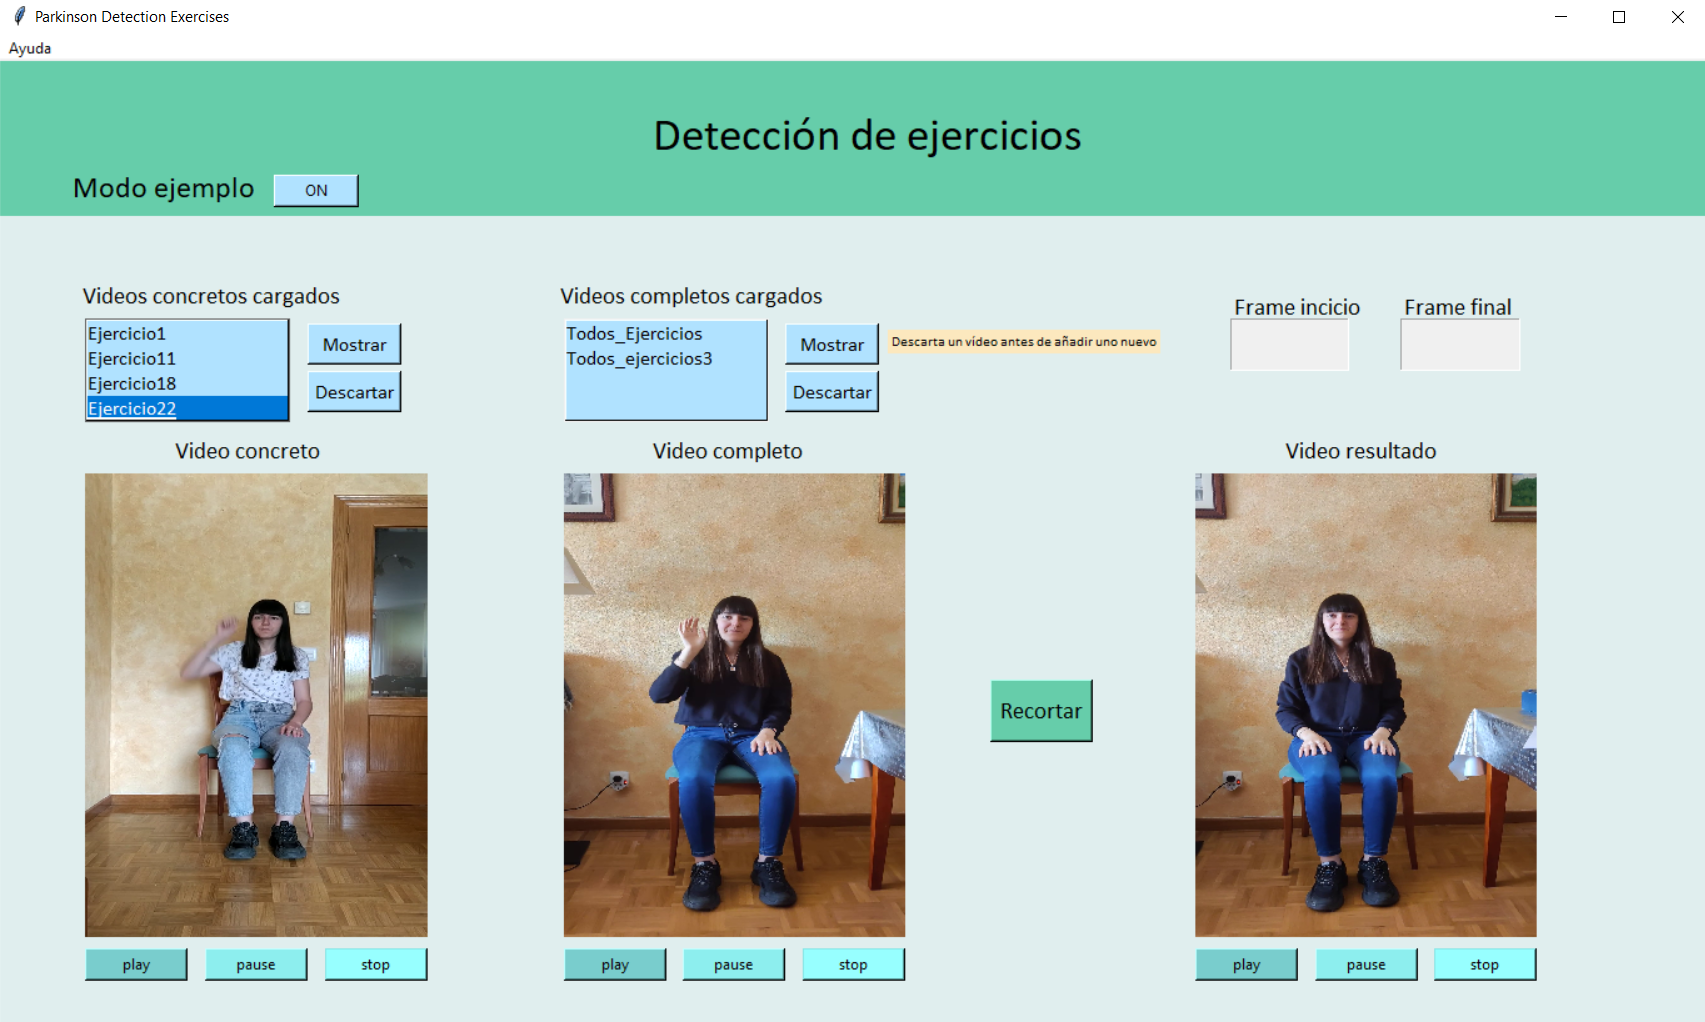
\includegraphics[width=\textwidth]{plantillaLatex-master/img/app5.PNG}
    \caption{Recorte de vídeos en modo ejemplo ON.}
    \label{fig:app5_}
\end{figure}

Un ejemplo de de la aplicación en \textbf{modo ejemplo ON} es el que se muestra en la figura \ref{fig:app5_}, mientras que un ejemplo de uso en \textbf{modo ejemplo OFF} correspondería con la figura \ref{fig:app4_}. En ambas se puede observar como se selecciona un vídeo concreto, un vídeo completo que contiene varios ejercicios, y el programa devuelve el ejercicio concreto que se localiza dentro del vídeo que contiene múltiples ejercicios.

Para finalizar, especificar que aunque esta parte del proyecto sea la más vistosa no es para nada la parte más relevante del proyecto ya que ha sido creada únicamente para mostrar los resultados. Esta aplicación podría ser usada por un terapeuta que ha obtenido múltiples secuencias de inicio y fin y quiere comprobar como de bien están realizando sus pacientes los ejercicios. Pero esta cuestión queda únicamente planteada ya que de momento el algoritmo no es lo suficientemente preciso como para que se comercialice. 

\section{Aspecto relevante}

Finalmente comentar en este apartado que todas las imágenes en las que aparecen individuos han sido obtenidas por medio de la web \textbf{Pixabay} que ofrece multitud de imágenes con gran calidad y sin derechos de autor, o han sido creadas por la autora del proyecto tras recibir el consentimiento de sus compañeros para mostrar sus vídeos e imágenes en este proyecto. 

